\section*{22. Smoothing Using Orthogonal Functions}\label{smoothing-using-orthogonal-functions}
In this Chapter we study a different approach to nonparametric curve
estimation based on \textbf{orthogonal functions}. We begin with a brief
introduction to the theory of orthogonal functions. Then we turn to
density estimation and regression.

\subsection*{\texorpdfstring{22.1 Orthogonal Functions and \(L_{2}\) Spaces}{22.1 Orthogonal Functions and L\_{2} Spaces}}\label{orthogonal-functions-and-l_{2}-spaces}
Let \(v = (v_{1}, v_{2}, v_{3})\) denote a three dimensional vector. Let
\(\mathcal{V}\) denote the set of all such vectors.
\begin{itemize}[tightlist]
\item
  If \(a\) is a scalar and \(v\) is a vector, we define
  \(av = (av_{1}, av_{2}, av_{3})\).
\item
  The sum of vectors \(v\) and \(w\) is defined as
  \(v + w = (v_{1} + w_{1}, v_{2} + w_{2}, v_{3} + w_{3})\).
\item
  The \textbf{inner product} between vectors \(v\) and \(w\) is defined
  by \(\langle v, w \rangle = \sum_{i} v_{i} w_{i}\).
\item
  The \textbf{norm} (or \textbf{length}) of a vector is defined by
\end{itemize}
\[
\Vert v \Vert = \sqrt{\langle v, v \rangle} = \sqrt{\sum_{i} v_{i}^{2} }
\]
\begin{itemize}[tightlist]
\item
  Two vectors are \textbf{orthogonal} (or \textbf{perpendicular}) if
  \(\langle v, w \rangle = 0\).
\item
  A set of vectors are orthogonal if each pair in the set is orthogonal.
\item
  A vector is \textbf{normal} if \(\Vert v \Vert = 1\).
\end{itemize}
Let \(\phi_{1} = (1, 0, 0)\), \(\phi_{2} = (0, 1, 0)\),
\(\phi_{3} = (0, 0, 1)\). These vectors are said to be an
\textbf{orthonormal basis} for \(\mathcal{V}\) since they have the
following properties:
\begin{itemize}[tightlist]
\item
  they are orthogonal
\item
  they are normal
\item
  they form a basis for \(\mathcal{V}\), that is, if
  \(v \in \mathcal{V}\) then \(v\) can be written as a linear
  combination of \(\phi_{i}\),
\end{itemize}
\[
v = \sum_{i} \beta_{i} \phi_{i}
\quad \text{where } \beta_{i} = \langle \phi_{i}, v \rangle
\]
There are other orthonormal basis for \(\mathcal{V}\), for example
\[
\psi_{1} = \left( \frac{1}{\sqrt{3}}, \frac{1}{\sqrt{3}} , \frac{1}{\sqrt{3}} \right),
\quad
\psi_{2} = \left( \frac{1}{\sqrt{2}}, -\frac{1}{\sqrt{2}} , 0 \right),
\quad
\psi_{3} = \left( \frac{1}{\sqrt{6}}, \frac{1}{\sqrt{6}} , -\frac{2}{\sqrt{6}} \right)
\]
Now we make the leap from vectors to functions. Basically, we just
replace vectors with functions and sums with integrals.
Let \(L_{2}(a, b)\) denote all functions defined on the interval
\([a, b]\) such that \(\int_a^{b} f(x)^{2} dx < \infty\):
\[
L_{2}(a, b) = \left\{ f: [a, b] \rightarrow \R , \int_a^{b} f(x)^{2} < \infty \right\}
\]
We sometimes write \(L_{2}\) instead of \(L_{2}(a, b)\).
\begin{itemize}[tightlist]
\item
  The inner product between two functions \(f, g \in L_{2}\) is
  \(\langle f, g \rangle = \int f(x) g(x) dx\).
\item
  The norm of \(f\) is
\end{itemize}
\[
\Vert f \Vert = \sqrt{\int f(x)^{2} dx}
\]
\begin{itemize}[tightlist]
\item
  Two functions are orthogonal if \(\langle f, g \rangle = 0\).
\item
  A function is normal if \(\Vert f \Vert = 1\).
\item
  A sequence of functions \(\phi_{1}, \phi_{2}, \phi_{3}, \dots\) is
  \textbf{orthonormal} if \(|| \phi_{i} || = 1\) for each \(i\) and
  \(\langle \phi_{i}, \phi_{j} \rangle = 0\) for \(i \neq j\).
\item
  An orthonormal sequence is \textbf{complete} if the only function that
  is orthogonal to each \(\phi_{i}\) is the zero function. In that case,
  the functions \(\phi_{1}, \phi_{2}, \phi_{3}, \dots\) for a basis, meaning
  that if \(f \in L_{2}\) then \(f\) can be written as
\end{itemize}
\[
f(x) = \sum_{j=1}^{\infty} \beta_{j} \phi_{j}(x)
\quad \text{where } \beta_{j} = \int_a^{b} f(x) \phi_{j}(x) dx
\]
\textbf{Parseval's relation} says that
\[
\Vert f \Vert^{2} \equiv \int f^{2}(x) dx = \sum_{j=1}^{\infty} \beta_{j}^{2} \equiv \Vert \beta \Vert^{2}
\]
The \textbf{cosine basis} is defined as follows: Let \(\phi_{1}(x) = 1\)
and for \(j \geq 2\) define
\[
\phi_{j}(x) = \sqrt{2} \cos \left( (j - 1) \pi x\right)
\]
The first ten functions are plotted below.

\begin{python}
import numpy as np
def cosine_basis(j):
    assert j >= 1
    
    def f(x):
        if j == 1:
            return np.ones_like(x)   
        return np.sqrt(2) * np.cos((j - 1) * np.pi * x)
    
    return f
\end{python}

\begin{python}
import matplotlib.pyplot as plt
step = 1e-3
xx = np.arange(0, 1 + step, step=step)
plt.figure(figsize=(12, 12))
for i in range(1, 11):
    
    # Set up the plot
    ax = plt.subplot(5, 2, i)
    ax.plot(xx, cosine_basis(i)(xx))
    ax.set_title('j = %i' % i)
plt.tight_layout()
plt.show()
\end{python}

\begin{figure}[H]
\centering
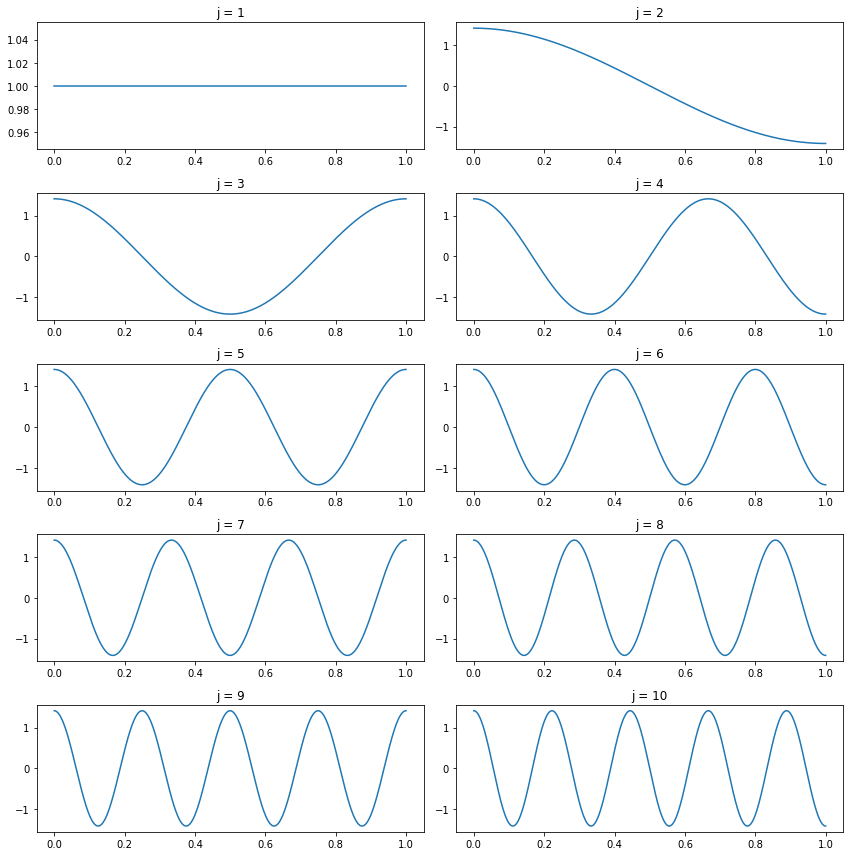
\includegraphics{Figure-22-01}
\end{figure}

The \textbf{Legendre polynomials} on \([-1, 1]\) are defined by
\[
P_{j}(x) = \frac{1}{2^{i} j!} \frac{d^{j}}{dx^{j}} (x^{2} - 1)^{j}, \quad j = 0, 1, 2, \dots
\]
It can be shown that these functions are complete and orthogonal, and
that
\[
\int_{-1}^{1} P_{j}^{2}(x) dx = \frac{2}{2j + 1}
\]
It follows that the functions
\[
\phi_{j}(x) = \sqrt{\frac{2j + 1}{2}}P_{j}(x), \quad j = 0, 1, 2, \dots
\]
form an orthonormal basis for \(L_{2}[-1, 1]\). The first few Legendre
polynomials are
\begin{align*}
P_{0}(x) &= 1 \\
P_{1}(x) &= x \\
P_{2}(x) &= \frac{1}{2}\left( 3x^{2} - 1 \right) \\
P_{3}(x) &= \frac{1}{2}\left( 5x^{3} - 3x \right)
\end{align*}
These polynomials may be constructed explicitly using the following
recursive relation:
\[
P_{j+1}(x) = \frac{(2j + 1) x P_{j}(x) - j P_{j - 1}(x)}{j + 1}
\]

\begin{python}
import sympy
from sympy.abc import x
from functools import lru_cache
@lru_cache(maxsize=None)
def legendre_polynomial(j):
    if j == 0:
        return 1
    if j == 1:
        return x
    
    return sympy.expand(((2*j - 1) * x * legendre_polynomial(j - 1) - (j - 1) * legendre_polynomial(j - 2)) / j)
def legendre_basis(j):
    if j == 0:
        return lambda x: np.sqrt(1/2) * np.ones_like(x)
    
    pj = legendre_polynomial(j)
    return sympy.lambdify(x, sympy.sqrt((2*j + 1) / 2) * pj, "numpy")
\end{python}

\begin{python}
import matplotlib.pyplot as plt
step = 1e-3
xx = np.arange(-1, 1 + step, step=step)
plt.figure(figsize=(12, 12))
for i in range(0, 10):
    
    # Set up the plot
    ax = plt.subplot(5, 2, i + 1)
    ax.plot(xx, legendre_basis(i)(xx))
    ax.set_title('j = %i' % i)
plt.tight_layout()
plt.show()
\end{python}

\begin{figure}[H]
\centering
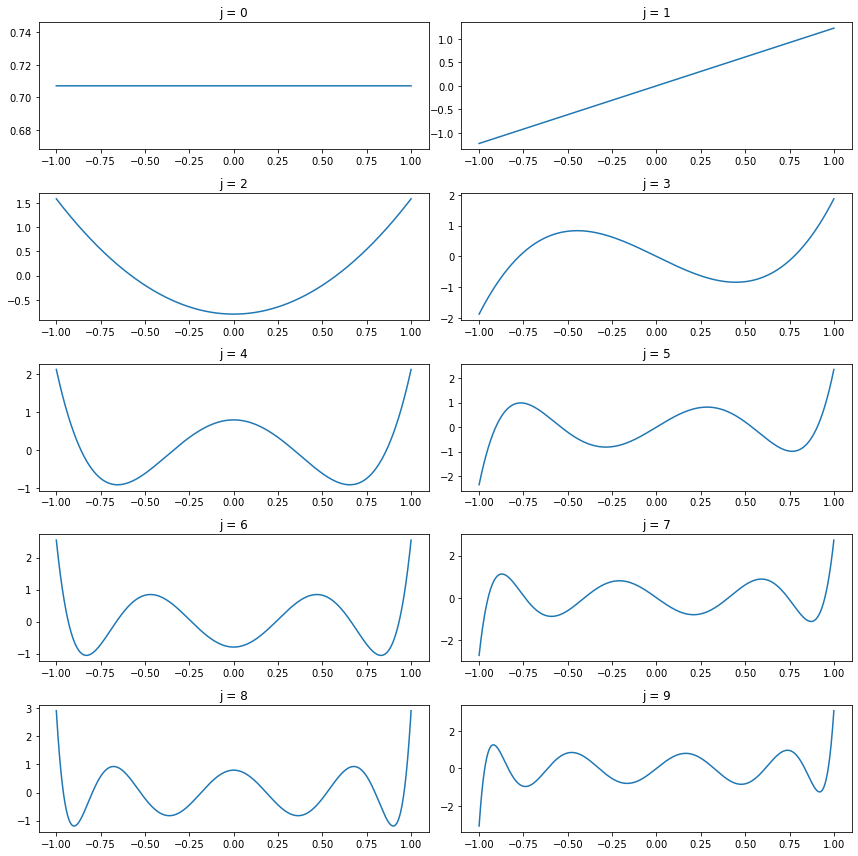
\includegraphics{Figure-22-02}
\end{figure}

The coefficients \(\beta_{1}, \beta_{2}, \dots\) are related to the
smoothness of the function \(f\). To see why note that, if \(f\) is
smooth, then its derivative will be finite. Thus we expect that, for
some \(k\), \(\int_{0}^{1} (f^{(k)}(x))^{2} dx < \infty\), where \(f^{(k)}\)
is the \(k\)-th derivative of \(f\).
Now consider the cosine basis and let
\(f(x) = \sum_{j=1}^{\infty} \beta_{j} \phi_{j}(x)\). Then,
\[
\int_{0}^{1} (f^{(k)}(x))^{2} dx = 2 \sum_{j=1}^{\infty} \beta_{j}^{2} ( \pi (j - 1) ) ^{2k}
\]
The only way the sum can be finite is if the \(\beta_{j}\)s get small
when \(j\) gets large. To summarize:
\textbf{If the function \(f\) is smooth then the coefficients
\(\beta_{j}\) will be small when \(j\) is large.}
For the rest of this chapter, we will assume we are using the cosine
basis unless otherwise specified.

\subsection*{22.2 Density Estimation}\label{density-estimation}
Let \(X_{1}, \dots, X_{n}\) be IID observations from a distribution on
\([0, 1]\) with density \(f\). Assuming \(f \in L_{2}\) we can write
\[
f(x) = \sum_{j=1}^{\infty} \beta_{j} \phi_{j}(x)
\]
where \(\phi_{i}\)s form an orthonormal basis. Define
\[
\hat{\beta}_{j} = \frac{1}{n} \sum_{i=1}^{n} \phi_{j}(X_{i})
\]

\textbf{Theorem 22.4}. The mean and variance of the \(\hat{\beta}_{j}\)
are
\[
\EXP(\hat{\beta}_{j}) = \beta_{j}
\quad \text{and} \quad
\VAR(\hat{\beta}_{j}) = \frac{\sigma_{j}^{2}}{n}
\]
where
\[
\sigma_{j}^{2} = \VAR(\phi_{j}(X_{i})) = \int \left( \phi_{j}(x) - \beta_{j}\right)^{2}f(x) dx
\]
\textbf{Proof}. We have
\[
\EXP(\hat{\beta}_{j}) = \frac{1}{n} \sum_{i=1}^{n} \EXP(\phi_{j}(X_{i})) = \EXP(\phi_{j}(X_{1}))  = \int \phi_{j}(x) f(x) dx = \beta_{j}
\]
The calculation for variance is similar:
\[
\VAR(\hat{\beta}_{j}) = \frac{1}{n^{2}} \sum_{i=1}^{n} \VAR(\phi_{j}(X_{i})) = \frac{1}{n} \VAR(\phi_{j}(X_{1})) = \frac{1}{n} \int \left( \phi_{j}(x) - \beta_{j}\right)^{2}f(x) dx
\]
Hence, \(\hat{\beta}_{j}\) is an unbiased estimate of \(\beta_{j}\). It is
tempting to estimate \(f\) by
\(\sum_{i=1}^{\infty} \hat{\beta}_{j} \phi_{j}(x)\) but it turns out to have a
very high variance. Instead, consider the estimator
\[
\hat{f}(x) = \sum_{i=1}^J \hat{\beta}_{j} \phi_{j}(x)
\]
The number of terms \(J\) is a smoothing parameter. Increasing \(J\)
will decrease bias while increasing variance. For technical reasons, we
restrict \(J\) to lie in the range \(1 \leq J \leq p\) where
\(p = p(n) = \sqrt{n}\). To emphasize the dependence of the risk
function on \(J\), we write the risk function as \(R(J)\).

\textbf{Theorem 22.5}. The risk of \(\hat{f}\) is given by
\[
R(J) = \sum_{j=1}^J \frac{\sigma_{j}^{2}}{J} + \sum_{j=J+1}^{\infty} \beta_{j}^{2}
\]
In kernel estimation, we used cross-validation to estimate the risk. In
the orthogonal function approach, we instead use the risk estimator
\[
\hat{R}(J) = \sum_{j=1}^J \frac{\hat{\sigma}_{j}^{2}}{n} + \sum_{j=J+1}^p \left( \hat{\beta}_{j}^{2} - \frac{\hat{\sigma}_{j}^{2}}{n} \right)_{+}
\]
where \(a_{+} = \max \{ a, 0 \}\) and
\[
\hat{\sigma}_{j}^{2} = \frac{1}{n - 1} \sum_{i=1}^{n} \left( \phi_{j}(X_{i}) - \hat{\beta}_{j}\right)^{2}
\]
To motivate this estimator, note that \(\hat{\sigma}_{j}^{2}\) is an
unbiased estimator of \(\sigma^{2}\) and
\(\hat{\beta}_{j}^{2} - \hat{\sigma}_{j}^{2} / n\) is an unbiased estimator of
\(\beta_{j}^{2}\). We take the positive part of the later term since we know
\(\beta_{j}^{2}\) cannot be negative. We now choose
\(1 \leq \hat{J} \leq p\) to minimize the risk estimator \(\hat{R}(J)\).
\textbf{Summary of Orthogonal Function Density Estimation}
\begin{enumerate}[tightlist,label={\arabic*.}]
\item
  Let
\end{enumerate}
\[
\hat{\beta}_{j} = \frac{1}{n} \sum_{i=1}^{n} \phi_{j}(X_{i})
\]
\begin{enumerate}[tightlist,label={\arabic*.}]
\item
  Choose \(\hat{J}\) to minimize \(\hat{R}(J)\) over
  \(1 \leq J \leq p = \sqrt{n}\) where
\end{enumerate}
\[
\hat{R}(J) = \sum_{j=1}^J \frac{\hat{\sigma}_{j}^{2}}{n} + \sum_{j=J+1}^p \left( \hat{\beta}_{j}^{2} - \frac{\hat{\sigma}_{j}^{2}}{n} \right)_{+}
\]
and
\[
\hat{\sigma}_{j}^{2} = \frac{1}{n - 1} \sum_{i=1}^{n} \left( \phi_{j}(X_{i}) - \hat{\beta}_{j}\right)^{2}
\]
\begin{enumerate}[tightlist,label={\arabic*.},resume]
\item
  Let
\end{enumerate}
\[
\hat{f}(x) = \sum_{j=1}^{\hat{J}} \hat{\beta}_{j} \phi_{j}(x)
\]
The estimator \(\hat{f}_{n}\) can be negative. If we are interested in
estimating the shape of \(f\), this is not a problem. However, if we
need the estimate to be a probability density function, we can truncate
the estimate and then normalize it:\\
\[
\hat{f}^{*}(x) = \frac{\max \{ \hat{f}_{n}(x), 0 \}}{\int_{0}^{1} \max \{ \hat{f}_{n}(u), 0 \} du}
\]
Now, let us construct a confidence band for \(f\). Suppose we estimate
\(f\) using \(J\) orthogonal functions. We are essentially estimating
\(\bar{f}(x) = \sum_{j=1}^J \beta_{j} \phi_{j}(x)\) instead of the true
density \(f(x) = \sum_{j=1}^{\infty} \beta_{j} \phi_{j}(x)\). Thus the
confidence band should be regarded as a band for \(\bar{f}(x)\).

\textbf{Theorem 22.6}. An approximate \(1 - \alpha\) confidence band for
\(\bar{f}\) is \((\ell(x), u(x))\) where
\[
\ell(x) = \hat{f}_{n}(x) - c
\quad \text{and} \quad
u(x) = \hat{f}_{n}(x) + x
\]
where
\[
c = \frac{JK^{2}}{\sqrt{n}} \sqrt{1 + \frac{\sqrt{2} z_{\alpha}}{\sqrt{J}}}
\]
and
\[
K = \max_{1 \leq j \leq J} \max_x | \phi_{j}(x) |
\]
For the cosine basis, \(K = \sqrt{2}\).

\subsection*{22.3 Regression}\label{regression}
Consider the regression model
\[
Y_{i} = r(x_{i}) + \epsilon_{i}, \quad i = 1, \dots, n
\]
where \(\epsilon_{i}\) are independent with mean 0 and variance
\(\sigma^{2}\). We will initially focus on the special case where
\(x_{i} = i / n\). We assume that \(r \in L_{2}[0, 1]\) and hence we can
write
\[
r(x) = \sum_{j=1}^{\infty} \beta_{j} \phi_{j}(x)
\quad \text{where } \beta_{j} = \int_{0}^{1} r(x) \phi_{j}(x) dx
\]
where \(\phi_{1}, \phi_{2}, \dots\) is an orthonormal basis for \([0, 1]\).
Define
\[
\hat{\beta}_{j} = \frac{1}{n} \sum_{i=1}^{n} Y_{i} \phi_{j}(x), 
\quad j = 1, 2, \dots
\]
Since \(\hat{\beta}_{j}\) is an average, the central limit Theorem tells
us that \(\hat{\beta}_{j}\) will be approximately normally distributed.

\textbf{Theorem 22.8}.
\[
\hat{\beta}_{j} \approx N \left( \beta_{j}, \frac{\sigma^{2}}{n} \right)
\]
\textbf{Proof}. The mean of \(\hat{\beta}_{j}\) is
\[
\EXP(\hat{\beta}_{j}) = \frac{1}{n} \sum_{i=1}^{n} \EXP(Y_{i}) \phi_{j}(x_{i}) = \frac{1}{n} \sum_{i=1}^{n} r(x_{i}) \phi_{j}(x_{i}) \approx \int r(x) \phi_{j}(x) dx = \beta_{j}
\]
where the approximate equality follows from the definition of a Riemann
integral: \(\sum_{i} h(x_{i}) / n \rightarrow \int_{0}^{1} h(x) dx\).
The variance is
\[
\VAR(\hat{\beta}_{j}) = \frac{1}{n^{2}} \sum_{i=1}^{n} \VAR(Y_{i}) \phi_{j}(x_{i}) = \frac{\sigma^{2}}{n} \left( \frac{1}{n} \sum_{i=1}^{n} \phi_{j}^{2}(x_{i}) \right) \approx \frac{\sigma^{2}}{n} \left( \int \phi_{j}^{2}(x) dx \right) = \frac{\sigma^{2}}{n}
\]
since \(\phi_{j}\) has norm 1.
As we did for density estimation, we will estimate \(r\) by
\[
\hat{r}(x) = \sum_{j=1}^J \hat{\beta}_{j} \phi_{j}(x)
\]
Let
\[
R(J) = \EXP \int (r(x) - \hat{r}(x))^{2} dx
\]
be the risk of the estimator.

\textbf{Theorem 22.9}. The risk \(R(J)\) of the estimator $ \hat{r}(x)
= \sum\_\{j=1\}^{J} \hat{\beta}\_{j} \phi\_{j}(x) $ is
\[
R(J) = \frac{J \sigma^{2}}{n} + \sum_{j=J+1}^{\infty} \beta_{j}^{2}
\]
To motivate the estimator \(\sigma^{2} = \VAR(\epsilon_{i})\) we use
\[
\hat{\sigma}^{2} = \frac{n}{k} \sum_{i=n - k + 1}^{n} \hat{\beta}_{j}^{2}
\]
where \(k = n / 4\). To motivate this estimator, recall that if \(f\) is
smooth then \(\beta_{j} \approx 0\) for large \(j\). So, for \(j \geq k\),
\(\hat{\beta}_{j} \approx N(0, \sigma^{2} / n)\). So
\(\hat{\beta}_{j} \approx \sigma Z_{j} / \sqrt{n}\) for \(j \geq k\), where
\(Z_{j} \sim N(0, 1)\). Therefore,
\[
\hat{\sigma}^{2} = \frac{n}{k} \sum_{i=n-k+1}^{k} \hat{\beta}_{j}^{2} \approx \frac{n}{k} \sum_{i=n-k+1}^{k} \left( \frac{\sigma}{\sqrt{n}} Z_{j} \right)^{2} = \frac{\sigma^{2}}{k} \sum_{i=n-k+1}^{k} Z_{j}^{2} = \frac{\sigma^{2}}{k} \chi_{k}^{2}
\]
since a sum of \(k\) squares of independent standard normals has a
\(\chi_{k}^{2}\) distribution. Now \(\EXP(\chi_{k}^{2}) = k\), leading to
\(\EXP(\hat{\sigma}^{2}) \approx \sigma^{2}\). Also,
\(\VAR(\chi_{k}^{2}) = 2k\) and so
\(\VAR(\hat{\sigma}^{2}) \approx (\sigma^{4} / k^{2}) 2k = 2\sigma^{4} / k \rightarrow 0\)
as \(n \rightarrow \infty\). Thus we expect \(\hat{\sigma}^{2}\) to be a
consistent estimator of \(\sigma^{2}\).
There is nothing special about the choice of \(k = n / 4\); any \(k\)
that increases with \(n\) at an appropriate rate would suffice.
We estimate the risk with
\[
\hat{R}(J) = J \frac{\hat{\sigma}^{2}}{n} + \sum_{j=J+1}^{n} \left(\hat{\beta}_{j}^{2} - \frac{\hat{\sigma}^{2}}{n} \right)_{+}
\]
We are now ready to give a complete description of the method which
Beran (2000) calls REACT (Risk Estimation and Adaptation by Coordinate
Transformation).
\textbf{Orthogonal Series Regression Estimator}
\begin{enumerate}[tightlist,label={\arabic*.}]
\item
  Let
\end{enumerate}
\[
\hat{\beta}_{j} = \frac{1}{n} \sum_{i=1}^{n} Y_{i} \phi_{i}(x_{i}), \quad j = 1, \dots, n
\]
\begin{enumerate}[tightlist,label={\arabic*.}]
\item
  Let
\end{enumerate}
\[
\hat{\sigma}^{2} = \frac{n}{k} \sum_{i=n-k+1}^{n} \hat{\beta}_{j}^{2}
\]
where \(k \approx n / 4\).
\begin{enumerate}[tightlist,label={\arabic*.},resume]
\item
  For \(1 \leq J \leq n\), compute the risk estimate
\end{enumerate}
\[
\hat{R}(J) = J \frac{\hat{\sigma}^{2}}{n} + \sum_{j=J+1}^{n} \left(\hat{\beta}_{j}^{2} - \frac{\hat{\sigma}^{2}}{n} \right)_{+}
\]
\begin{enumerate}
\def\labelenumi{\arabic{enumi}.}
\setcounter{enumi}{3}
\item
  Choose \(\hat{J} \in \{1, \dots, n \}\) to minimize \(\hat{R}(J)\).
\item
  Let
\end{enumerate}
\[
\hat{f}(x) = \sum_{j=1}^J \hat{\beta}_{j} \phi_{j}(x)
\]
Finally, we turn to confidence bands. As before, these bands are not for the true regression function \(r(x)\), but for the smoothed version of the function
\(\bar{r}(x) = \sum_{i=1}^{\bar{J}} \beta_{j} \phi_{j}(x)\).

\textbf{Theorem 22.11}. Suppose the estimate \(\hat{r}\) is based on
\(J\) terms and $\hat{\sigma}^{2} = \frac{n}{k} \sum\_\{i=n-k+1\}^{n}
\hat{\beta}\_{j}^{2} $. Assume that \(J < n - k + 1\). An approximate
\(1 - \alpha\) confidence band for \(\bar{r}\) is \((\ell, u)\),
where
\[
\ell(x) = \hat{r}(x) - K \sqrt{J} \sqrt{\frac{z_{\alpha} \hat{\tau}}{\sqrt{n}} + \frac{J \hat{\sigma}^{2}}{n}}
\quad \text{and} \quad u(x) = \hat{r}(x) + K \sqrt{J} \sqrt{\frac{z_{\alpha} \hat{\tau}}{\sqrt{n}} + \frac{J \hat{\sigma}^{2}}{n}}
\]
where
\[
K = \max_{1 \leq j \leq J} \max_x | \phi_{j}(x) |
\]
and
\[
\hat{\tau}^{2} = \frac{2 J \hat{\sigma}^{4}}{n} \left( 1 + \frac{J}{k} \right)
\]
and \(k = n / 4\) as used in the definition of \(\hat{\sigma}^{2}\). In
the cosine basis, \(K = \sqrt{2}\).
So far, we have assumed that the \(x_{i}\) are of the form
\(\{1/n, 2/n, \dots, 1\}\). If \(x_{i} \in [a, b]\) then we can rescale
them to be in \([0, 1]\). If the \(x_{i}\)s are not equally spaced the
methods discussed here apply as long as they ``fill out'' the interval
in a way as to not be too clumped together. If we want to treat the
\(x_{i}\)s as random instead of fixed, then the method needs significant
modifications which will not be treated here.

\subsection*{22.4 Wavelets}\label{wavelets}
Suppose there is a sharp jump in a regression function \(f\) at some
point \(x\) but that \(f\) is otherwise very smooth. Such as function is
said to be \textbf{spatially inhomogeneous}.

\begin{python}
import numpy as np
from scipy.stats import norm
import matplotlib.pyplot as plt
%matplotlib inline
xx = np.arange(0, 1, step=1e-3)
plt.figure(figsize=(12, 8))
plt.plot(xx, norm.pdf(xx, loc=0.65, scale=0.5) + 1e-2 * norm.pdf(xx, loc=0.45, scale=0.01))
plt.show()
\end{python}

\begin{figure}[H]
\centering
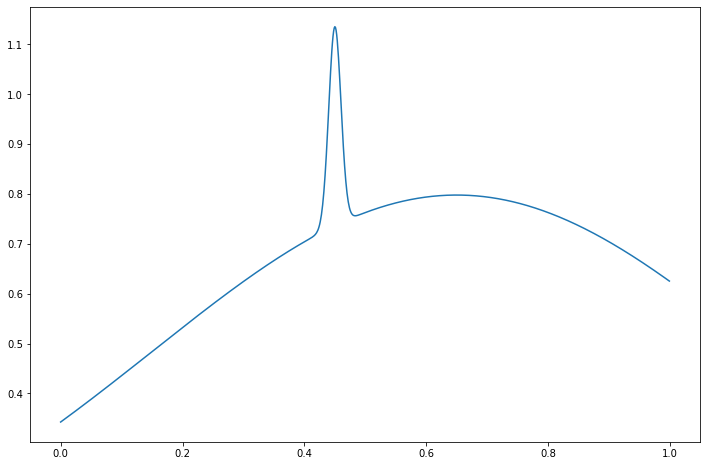
\includegraphics{Figure-22-03}
\end{figure}

It is hard to estimate \(f\) using the methods we discussed so far. If we
use a cosine basis and only keep the low order terms, we will miss the
peak; if we allow higher order terms we will find the peak but we will
make the rest of the curve very wiggly. Similar comments apply to kernel
regression: if we use a large bandwidth, then we will smooth out the
peak; if we use a small bandwidth, then we will find the peak but we
will make the rest of the curve very wiggly.
One way to estimate inhomogeneous functions is to use a more carefully
chosen basis that allows us to place a ``blip'' in some small region
without adding wiggles elsewhere. In this section, we describe a special
class of bases called \textbf{wavelets} that are aimed at fixing this
problem. Statistical inference using wavelets is a large and active
area. We will just discuss a few ideas to get a flavor of this approach.
The \textbf{father Haar wavelet} of \textbf{Haar scaling function} is
defined by
\[
\phi(x) = \begin{cases}
1 & \text{if } 0 \leq x < 1 \\
0 & \text{otherwise}
\end{cases}
\]
The \textbf{mother Haar wavelet} is defined by
\[
\psi(x) = \begin{cases}
-1 & \text{if } 0 \leq x \leq \frac{1}{2} \\
1  & \text{if } \frac{1}{2} < x \leq 1
\end{cases}
\]
For any integers \(j\) and \(k\) define
\[
\phi_{j, k}(x) = 2^{j/2} \phi(2^{j} x - k) 
\quad \text{and} \quad
\psi_{j, k}(x) = 2^{j/2} \psi(2^{j} x - k)
\]
The function \(\psi_{j, k}\) has the same shape as \(\psi\) but it has
been rescaled by a factor of \(2^{j/2}\) and shifted by a factor of
\(k\).

\begin{python}
import numpy as np
def haar_father_wavelet(x):
    return np.where((x >= 0) & (x < 1), 1, 0)
def haar_mother_wavelet(x):
    return np.where((x >= 0) & (x < 1),  np.where(x <= 1/2, -1, 1), 0)
def phi_wavelet(j, k):
    def f(x):
        return 2**(j / 2) * haar_father_wavelet((2**j)*x - k)
    return f
def psi_wavelet(j, k):
    def f(x):
        return 2**(j / 2) * haar_mother_wavelet((2**j)*x - k)
    return f
\end{python}

\begin{python}
import matplotlib.pyplot as plt
step = 1e-4
xx = np.arange(0, 1, step=step)
plt.figure(figsize=(12, 8))
ax = plt.subplot(2, 2, 1)
ax.plot(xx, haar_father_wavelet(xx))
ax.set_title(r'Father wavelet $\phi$')
    
ax = plt.subplot(2, 2, 2)
ax.plot(xx, haar_mother_wavelet(xx))
ax.set_title(r'Mother wavelet $\psi$')
ax = plt.subplot(2, 2, 3)
ax.plot(xx, psi_wavelet(2, 2)(xx))
ax.set_title(r'$\psi_{2, 2}$')
ax = plt.subplot(2, 2, 4)
ax.plot(xx, psi_wavelet(4, 10)(xx))
ax.set_title(r'$\psi_{4, 10}$')
plt.tight_layout()
plt.show()
\end{python}

\begin{figure}[H]
\centering
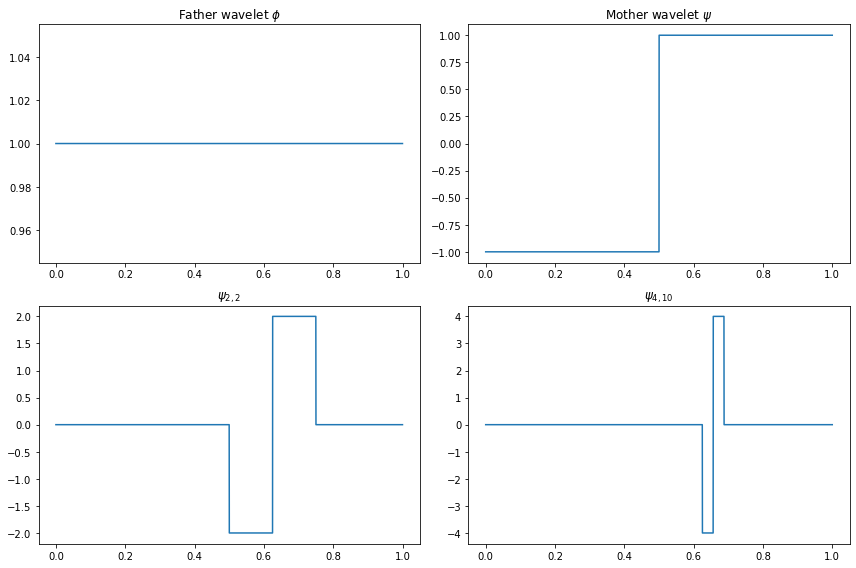
\includegraphics{Figure-22-04}
\end{figure}

Notice that for large \(j\), \(\psi_{j, k}\) is a very localized
function. This makes it possible to add a blip to a function without
adding wiggles elsewhere. In technical terms, we say that wavelets
provide a \textbf{multiresolution analysis} of \(L_{2}(0, 1)\).
Let
\[
W_{j} = \{\psi_{j, k}, \; k = 0, 1, \dots, 2^{j} - 1\}
\]
be the set of rescaled and shifted mother wavelets at resolution \(j\).

\textbf{Theorem 22.13}. The set of functions
\[
\left\{ \phi, W_{0}, W_{1}, W_{2}, \dots \right\}
\]
is an orthonormal basis for \(L_{2}(0, 1)\).
It follows from this Theorem that we can expand any function
\(f \in L_{2}(0, 1)\) in this basis. Because each \(W_{j}\) is itself a set
of functions, we write the expansion as a double sum:
\[
f(x) = \alpha \phi(x) + \sum_{j=0}^{\infty} \sum_{k=0}^{2^{j} - 1} \beta_{j, k} \psi_{j, k}(x)
\]
where
\[
\alpha = \int_{0}^{1} f(x) \phi(x) dx, \quad \beta_{j, k} = \int_{0}^{1} f(x) \psi_{j, k}(x) dx
\]
We call \(\alpha\) the \textbf{scaling coefficient} and \(\beta_{j, k}\)
the \textbf{detail coefficients}. We call the finite sum
\[
\bar{f}(x) = \alpha \phi(x) + \sum_{j=0}^{J - 1} \sum_{k=0}^{2^{j} - 1} \beta_{j, k}
\]
the \textbf{resolution \(J\)} approximation to \(f\). The total number
of terms in this sum is
\[
1 + \sum_{j=0}^{J - 1}2^{j} = 2^J
\]
Haar wavelets are localized, meaning they are zero outside of an
interval, but they are not smooth. In 1988, Ingrid Daubechie showed that
such wavelets do exist. They can be constructed numerically, but there
is no closed form formula for smoother wavelets. To keep things simple,
we will continue to use Haar wavelets.
We can now use wavelets to do density estimation and regression. We
shall only discuss the regression problem
\(Y_{i} = r(x_{i}) + \sigma \epsilon_{i}\) where \(\epsilon_{i} \sim N(0, 1)\)
and \(x_{i} = i / n\). To simplify this discussion we assume that
\(n = 2^J\) for some \(J\).
There is one major difference between estimation using wavelets instead
of a cosine (or polynomial) basis. With the cosine basis, we used all
terms \(1 \leq j \leq J\) for some \(J\). With wavelets, we use a method
called \textbf{thresholding} where we keep a term in the function
approximation only if its coefficient is large. The simplest version is
called hard, universal threshold.
\textbf{Haar Wavelet Regression}
\begin{enumerate}[tightlist,label={\arabic*.}]
\item
  Let \(J = \log_{2} n\) and define
\end{enumerate}
\[
\hat{\alpha} = \frac{1}{n} \sum_{i} \phi(x_{i}) Y_{i}
\quad \text{and} \quad
D_{j, k} = \frac{1}{n} \sum_{i} \psi_{j, k}(x_{i}) Y_{i}
\]
for \(0 \leq j \leq J - 1\)
\begin{enumerate}[tightlist,label={\arabic*.}]
\item
  Estimate \(\sigma\) by
\end{enumerate}
\[
\hat{\sigma} = \sqrt{n} \; \times \; \frac{\text{median} \left( \left| D_{J-1, k} : k = 0, \dots, 2^{J - 1} - 1\right| \right)}{0.6745}
\]
\begin{enumerate}[tightlist,label={\arabic*.},resume]
\item
  Apply universal thresholding:
\end{enumerate}
\[
\hat{\beta}_{j, k} = \begin{cases}
D_{j, k} & \text{if } \left| D_{j, k} \right| > \hat{\sigma} \sqrt{\frac{2 \log n}{n}} \\
0 & \text{otherwise}
\end{cases}
\]
\begin{enumerate}[tightlist,label={\arabic*.},resume]
\item
  Set
\end{enumerate}
\[
\hat{f}(x) = \hat{\alpha} \phi(x) + \sum_{j = j_{0}}^{J - 1} \sum_{k = 0}^{2^{j} - 1} \hat{\beta}_{j, k} \psi_{j, k}(x)
\]
In practice, we do not compute \(\hat{\alpha}\) and \(D_{j, k}\).
Instead, we use the \textbf{discrete wavelet transform (DWT)} which is
very fast. For Haar wavelets, the DWT works as follows.
\textbf{DWT for Haar Wavelets}
\begin{itemize}[tightlist]
\item
  Let \(y = (Y_{1}, \dots, Y_{n})\) and let \(J = \log_{2} n\).\\
\item
  Create a list \(D\) with elements \(D[0], ..., D[J - 1]\)
\item
  Do:
\end{itemize}
\begin{console}
temp <- y / sqrt(n)
for j in (J - 1):0 {
  m <- 2^{j}
  I <- (1:m)
  D[j] <- (temp[2 * I] - temp[(2 * I) - 1]) / sqrt(2)
  temp <- (temp[2 * I] + temp[(2 * I) - 1]) / sqrt(2)
}
\end{console}
The estimate used for \(\sigma\) probably looks strange. It is similar
to the estimate used for the cosine basis but it is designed to be
insensitive to sharp peaks in the function.
To understand the intuition behind universal thresholding, consider what
happens when there is no signal, that is, when \(\beta_{j, k} = 0\) for
all \(j, k\).

\textbf{Theorem 22.16}. Suppose that \(\beta_{j, k} = 0\) for all
\(j, k\) and let \(\hat{\beta}_{j, k}\) be the universal threshold
estimator. Then
\[
\PROB\left(\hat{\beta}_{j, k} = 0 \; \text{for all } j, k \right) \rightarrow 1
\]
as \(n \rightarrow \infty\).
\textbf{Proof} Assume \(\sigma\) is known. Now
\(D_{j, k} \approx N(0, \sigma^{2} / n)\). We will need \textbf{Mill's
inequality}: if \(Z \sim N(0, 1)\) then
\(\PROB(|Z| > t) \leq (c / t) e^{-t^{2} / 2}\) where
\(c = \sqrt{2 / pi}\) is a constant. Thus,
\begin{align*}
\PROB(\max |D_{j, k}| > \lambda) &\leq \sum_{j, k} \PROB(|D_{j, k}| > \lambda) \\
& \leq \sum_{j, k} \PROB \left( \frac{\sqrt{n} |D_{j, k}|}{\sigma} > \frac{\sqrt{n} \lambda}{\sigma} \right) \\
& \leq \sum_{j, k} \frac{c \sigma}{\lambda \sqrt{n}} \exp \left\{ - \frac{1}{2} \frac{n \lambda^{2}}{\sigma^{2}} \right\} \\
& = \frac{c}{\sqrt{2 \log n}} \rightarrow 0
\end{align*}

\subsection*{22.6 Exercises}

\textbf{Exercise 22.6.1}. Prove Theorem 22.5.
The risk of \(\hat{f}\) is given by
\[
R(J) = \sum_{j=1}^J \frac{\sigma_{j}^{2}}{n} + \sum_{j=J+1}^{\infty} \beta_{j}^{2}
\]

\textbf{Solution}.
The density estimator \(\hat{f}\) is defined as
\[
\hat{f}(x) = \sum_{i=1}^J \hat{\beta}_{j} \phi_{j}(x) 
\quad \text{where} \quad
\hat{\beta}_{j} = \frac{1}{n} \sum_{i=1}^{n} \phi_{j}(X_{i})
\]
From Theorem 22.4,
\[
\EXP[\hat{\beta}_{j}] = \beta_{j}
\quad \text{and} \quad
\VAR[\hat{\beta}_{j}] = \frac{\sigma_{j}^{2}}{n}
\]
The (unintegrated) variance is
\[
\VAR[f(x) - \hat{f}(x)] = \VAR[\hat{f}(x)] 
= \sum_{j=1}^J \VAR[\hat{\beta}_{j}]\phi_{j}(x)^{2} + 2 \sum_{i < j} \COV(\hat{\beta}_{i}, \hat{\beta}_{j}) \phi_{i}(x) \phi_{j}(x)
\]
so, integrating,
\begin{align*}
\int \VAR[f(x) - \hat{f}(x)] dx &= \sum_{j=1}^J \VAR[\hat{\beta}_{j}] \int \phi_{j}(x)^{2} dx + 2 \sum_{i < j} \COV(\hat{\beta}_{i}, \hat{\beta}_{j}) \int \phi_{i}(x) \phi_{j}(x) dx  \\
&= \sum_{j=1}^J \VAR[\hat{\beta}_{j}] \langle \phi_{j}, \phi_{j} \rangle + 2 \sum_{i < j} \COV(\hat{\beta}_{i}, \hat{\beta}_{j}) \langle \phi_{i}, \phi_{j} \rangle \\
&= \sum_{j=1}^J \VAR[\hat{\beta}_{j}] = \sum_{j=1}^J \frac{\sigma_{j}^{2}}{n}
\end{align*}
while the integrated expected bias squared is:
\begin{align*}
\int \EXP\left[\left(f(x) - \hat{f}(x)\right)^{2}\right] dx
&= \int \EXP\left[\left(\sum_{j=1}^{\infty} \beta_{j} \phi_{j}(x) - \sum_{j=1}^J \hat{\beta}_{j} \phi_{j}(x)\right)^{2}\right] dx 
\\
&= \int \EXP \left[ \left(\sum_{j=1}^{\infty} \beta_{j} \phi_{j}(x)\right)^{2} \right] dx
\\&\quad
+ \int \EXP \left[ \left(\sum_{j=1}^J \hat{\beta}_{j} \phi_{j}(x)\right)^{2} \right] dx
\\&\quad
- \int \EXP \left[ \sum_{i=1}^{\infty} \sum_{j=1}^J \beta_{i} \hat{\beta}_{j} \phi_{i}(x) \phi_{j}(x) \right] dx 
\\
&= \sum_{j=1}^{\infty} \beta_{j}^{2} \int \phi_{j}(x)^{2} dx 
+ \sum_{j=1}^J \beta_{j}^{2} \int \phi_{j}(x)^{2} dx 
- 2 \sum_{j=1}^J \beta_{j}^{2} \int \phi_{j}(x)^{2} dx 
\\
&= \sum_{j=J+1}^{\infty} \beta_{j}^{2}
\end{align*}
since
\(\langle \phi_{i}, \phi_{j} \rangle = \int \phi_{i}(x) \phi_{j}(x) dx = 0\) for
\(i \neq j\), and since
\(\langle \phi_{j}, \phi_{j} \rangle = \int \phi_{j}(x)^{2} dx = 1\).
Then, the risk is the bias squared plus the variance,
\[
R(J) = \sum_{j=1}^J \frac{\sigma_{j}^{2}}{n} + \sum_{j=J+1}^{\infty} \beta_{j}^{2}
\]
as desired.

\textbf{Exercise 22.6.2}. Prove Theorem 22.9.
The risk \(R(J)\) of the estimator $ \hat{r}(x) = \sum\_\{j=1\}^{J}
\hat{\beta}\_{j} \phi\_{j}(x) $ is
\[
R(J) = \frac{J \sigma^{2}}{n} + \sum_{j=J+1}^{\infty} \beta_{j}^{2}
\]

\textbf{Solution}. Consider the probability distribution function
obtained by shifting the true regression function to a minimum of 0, and
rescaled to integrate to 1:
\[
f(x) = \frac{r(x) - r_{0}}{A} \quad \text{where } A = \int r(y) dy - r_{0}, r_{0} = \inf_x r(x)
\]
But if \(r(x) = \sum_{j=1}^{\infty} \beta_{j} \phi_{j}(x)\), then
\[
f(x) = -\frac{r_{0}}{A} + \sum_{j=1}^{\infty} \left( \frac{\beta_{j}}{A} \right) \phi_{j}(x) = \sum_{j=1}^{\infty} \left( \frac{\beta_{j}}{A} + c_{j} \right) \phi_{j}(x)
\]
where the \(c_{j}\)s are the decomposition of the constant function
\(-r_{0} / A\) on the basis of the functions \(\phi_{j}\)s. Assuming a
sensible basis, \(\phi_{0}\) is constant and \(c_{j} = 0\) for \(j > 1\).
By Theorem 22.5, the risk of the PDF estimation is
\[
\sum_{j=1}^J \frac{\sigma_{j}^{2}}{n} + \sum_{j=J+1}^{\infty} \left( \frac{\beta_{j}}{A} \right)^{2} = \frac{1}{A^{2}} \left( \frac{J \sigma^{2}}{n} + \sum_{j=J+1}^{\infty} \beta_{j}^{2} \right)
\]
and so the result follows.

\textbf{Exercise 22.6.3}. Let
\[
\psi_{1} = \left( \frac{1}{\sqrt{3}}, \frac{1}{\sqrt{3}} , \frac{1}{\sqrt{3}} \right),
\quad
\psi_{2} = \left( \frac{1}{\sqrt{2}}, -\frac{1}{\sqrt{2}} , 0 \right),
\quad
\psi_{3} = \left( \frac{1}{\sqrt{6}}, \frac{1}{\sqrt{6}} , -\frac{2}{\sqrt{6}} \right)
\]
Show that these vectors have norm 1 and are orthogonal.

\textbf{Solution}. Results follow from inspection.
Norms:
\begin{align*}
\langle \psi_{1}, \psi_{1} \rangle 
&= \frac{1}{\sqrt{3}} \cdot \frac{1}{\sqrt{3}} + \frac{1}{\sqrt{3}} \cdot \frac{1}{\sqrt{3}} + \frac{1}{\sqrt{3}} \cdot \frac{1}{\sqrt{3}} 
\\
&= \frac{1}{3} + \frac{1}{3} + \frac{1}{3} 
\\
&= 1 
\\
\langle \psi_{2}, \psi_{2} \rangle 
&= \frac{1}{\sqrt{2}} \cdot \frac{1}{\sqrt{2}} + \frac{-1}{\sqrt{2}} \cdot \frac{-1}{\sqrt{2}} + 0 \cdot 0 
\\
&= \frac{1}{2} + \frac{1}{2} + 0 
\\
&= 1 
\\
\langle \psi_{3}, \psi_{3} \rangle 
&= \frac{1}{\sqrt{6}} \cdot \frac{1}{\sqrt{6}} + \frac{1}{\sqrt{6}} \cdot \frac{1}{\sqrt{6}} + \frac{-2}{\sqrt{6}} \cdot \frac{-2}{\sqrt{6}}
\\ 
&= \frac{1}{6} + \frac{1}{6} + \frac{4}{6} 
\\
&= 1
\end{align*}
Orthogonality: \begin{align*}
\langle \psi_{1}, \psi_{2} \rangle 
&= \frac{1}{\sqrt{3}} \cdot \frac{1}{\sqrt{2}} + \frac{1}{\sqrt{3}} \cdot \frac{-1}{\sqrt{2}} + \frac{1}{\sqrt{3}} \cdot 0 
\\
&= \frac{1}{\sqrt{6}} + \frac{-1}{\sqrt{6}} + 0 
\\
&= 0 
\\
\langle \psi_{1}, \psi_{3} \rangle 
&= \frac{1}{\sqrt{3}} \cdot \frac{1}{\sqrt{6}} + \frac{1}{\sqrt{3}} \cdot \frac{1}{\sqrt{6}} + \frac{1}{\sqrt{3}} \cdot \frac{-2}{\sqrt{6}} 
\\
&= \frac{1}{3\sqrt{2}} + \frac{1}{3\sqrt{2}} + \frac{-2}{3\sqrt{2}} 
\\
&= 0 
\\
\langle \psi_{2}, \psi_{3} \rangle 
&= \frac{1}{\sqrt{2}} \cdot \frac{1}{\sqrt{6}} + \frac{-1}{\sqrt{2}} \cdot \frac{1}{\sqrt{6}} + 0 \cdot \frac{-2}{\sqrt{6}} 
\\
&= \frac{1}{2\sqrt{3}} + \frac{-1}{2\sqrt{3}} + 0 
\\
&= 0 
\end{align*}

\textbf{Exercise 22.6.4}. Prove Parseval's relation equation.
\[
\Vert f \Vert^{2} \equiv \int f^{2}(x) dx = \sum_{j=1}^{\infty} \beta_{j}^{2} \equiv \Vert \beta \Vert^{2}
\]

\textbf{Solution}. We have:
\begin{align*}
\int f^{2}(x) dx &= \int \left( \sum_{i=1}^{\infty} \beta_{i} \phi_{i}(x) \right)^{2} dx \\
&= \int \left( \sum_{i=1}^{\infty} \beta_{i}^{2} \phi_{i}^{2}(x) + \sum_{i=1}^{\infty} \sum_{j=1, j \neq i}^{\infty} \beta_{i} \beta_{j} \phi_{i}(x) \phi_{j}(x) \right) dx \\
&= \sum_{i=1}^{\infty} \beta_{i}^{2} \int \phi_{i}^{2}(x) dx + \sum_{i=1}^{\infty} \sum_{j=1, j \neq i}^{\infty} \beta_{i} \beta_{j}  \int \phi_{i}(x) \phi_{j}(x) dx \\
&= \sum_{i=1}^{\infty} \beta_{i}^{2} \langle \phi_{i}, \phi_{i} \rangle + \sum_{i=1}^{\infty} \sum_{j=1, j \neq i}^{\infty} \beta_{i} \beta_{j} \langle \phi_{i}, \phi_{j} \rangle \\
&= \sum_{i=1}^{\infty} \beta_{i}^{2}
\end{align*}
since \(\langle \phi_{i}, \phi_{i} \rangle = 1\) and
\(\langle \phi_{i}, \phi_{j} \rangle = 0\) for \(i \neq j\).

\textbf{Exercise 22.6.5}. Plot the first five Legendre polynomials.
Verify, numerically, that they are orthonormal.

\textbf{Solution}.

\begin{python}
import sympy
from sympy.abc import x
from functools import lru_cache
@lru_cache(maxsize=None)
def legendre_polynomial(j):
    if j == 0:
        return 1
    if j == 1:
        return x
    
    return sympy.expand(((2*j - 1) * x * legendre_polynomial(j - 1) 
                        - (j - 1) * legendre_polynomial(j - 2)) / j)
def legendre_basis(j):
    if j == 0:
        return lambda x: np.sqrt(1/2) * np.ones_like(x)
    
    pj = legendre_polynomial(j)
    return sympy.lambdify(x, sympy.sqrt((2*j + 1) / 2) * pj, "numpy")
\end{python}

\begin{python}
import matplotlib.pyplot as plt
step = 1e-4
xx = np.arange(-1, 1 + step, step=step)
plt.figure(figsize=(12, 12))
for i in range(0, 5):
    
    # Set up the plot
    ax = plt.subplot(5, 1, i + 1)
    ax.plot(xx, legendre_basis(i)(xx))
    ax.set_title(r'Legendre Basis $\phi_%i$' % i)
plt.tight_layout()
plt.show()
\end{python}

\begin{figure}[H]
\centering
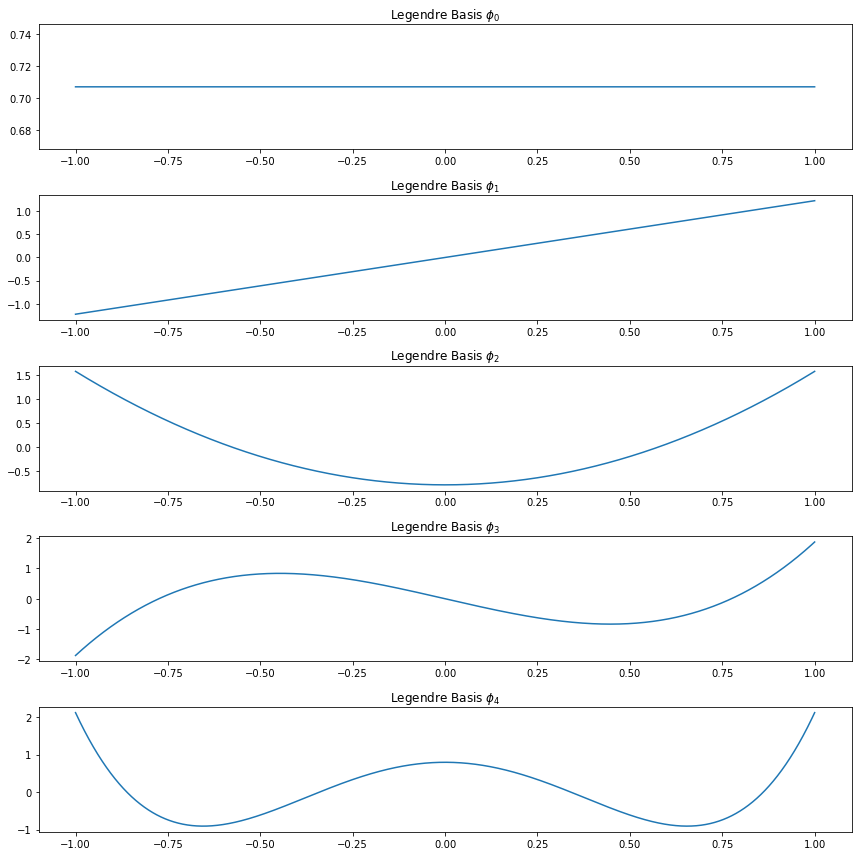
\includegraphics{Figure-22-05}
\end{figure}


\begin{python}
# Verifying orthogonality numerically
for i in range(0, 5):
    for j in range(i,5):
        product = legendre_basis(i)(xx) @ legendre_basis(j)(xx) * step
        print("<phi_%i, phi_%i>: %.3f" % (i, j, product))
\end{python}
\begin{console}
<phi\_{0}, phi\_{0}>: 1.000
<phi\_{0}, phi\_{1}>: -0.000
<phi\_{0}, phi\_{2}>: 0.000
<phi\_{0}, phi\_{3}>: -0.000
<phi\_{0}, phi\_{4}>: 0.000
<phi\_{1}, phi\_{1}>: 1.000
<phi\_{1}, phi\_{2}>: -0.000
<phi\_{1}, phi\_{3}>: 0.000
<phi\_{1}, phi\_{4}>: -0.000
<phi\_{2}, phi\_{2}>: 1.000
<phi\_{2}, phi\_{3}>: -0.000
<phi\_{2}, phi\_{4}>: 0.000
<phi\_{3}, phi\_{3}>: 1.000
<phi\_{3}, phi\_{4}>: -0.000
<phi\_{4}, phi\_{4}>: 1.000
\end{console}

\textbf{Exercise 22.6.6}. Expand the following functions in the cosine
basis on \([0, 1]\). For (a) and (b), find the coefficients \(\beta_{j}\)
analytically. For (c) and (d), find the coefficients \(\beta_{j}\)
numerically, i.e.
\[
\beta_{j} = \int_{0}^{1} f(x) \phi_{j}(x) \approx \frac{1}{N} \sum_{r=1}^N f \left( \frac{r}{N} \right) \phi_{j} \left( \frac{r}{N} \right)
\]
for some large integer \(N\). Then plot the partial sum
\(\sum_{j=1}^{n} \beta_{j} \phi_{j}(x)\) for increasing values of \(n\).
\textbf{(a)} \(f(x) = \sqrt{2} \cos (3 \pi x)\)
\textbf{(b)} \(f(x) = \sin(\pi x)\)
\textbf{(c)} \(f(x) = \sum_{j=1}^{11} h_{j} K(x - t_{j})\), where
\(K(t) = (1 + \text{sign}(t)) / 2\),
\[
(t_{j}) = (.1, .13, .15, .23, .25, .40, .44, .65, .76, .78, .81), \\
(h_{j}) = (4, -5, 3, -4, 5, -4.2, 2.1, 4.3, -3.1, 2.1, -4.2)
\]
\textbf{(d)} $f(x) = \sqrt{x(1-x)} \sin \left(
\frac{2.1 \pi}{(x + .05)} \right) $

\textbf{Solution}.
\textbf{(a)} is immediate by inspection:
\[
f(x) = \sqrt{2} \cos(3 \pi x) = \sum_{j=1}^{\infty} \beta_{j} \phi_{j}(x), \quad \text{where } \phi_{j}(x) = \sqrt{2} \cos((j - 1) \pi x)
\]
so
\[
\beta_{j} = \begin{cases}
1 & \text{if } j = 4 \\
0 & \text{otherwise}
\end{cases}
\]

\begin{python}
import numpy as np
def beta_{j}(j):
    if j == 4:
        return 1
    return 0
def phi_{j}(j):
    def f(x):
        if j == 1:
            return np.ones_like(x)
        return np.sqrt(2) * np.cos((j - 1) * np.pi * x)
    return f
def partial_sum(n, x):
    lx = len(x)
    terms = np.empty((n, lx))
    for j in range(1, n + 1):
        terms[j - 1] = beta_{j}(j) * phi_{j}(j)(xx)
    return terms.sum(axis = 0)
\end{python}

\begin{python}
# Plot in separate boxes for ease of visualization
import matplotlib.pyplot as plt
%matplotlib inline
step = 1e-4
xx = np.arange(0, 1 + step, step=step)
plt.figure(figsize=(12, 12))
def do_subplot(index, xx, yy, label, color):
    ax = plt.subplot(4, 1, index)
    ax.plot(xx, yy, label=label, color=color)
    ax.legend()    
do_subplot(1, xx, partial_sum(3,  xx), label=r'$n \leq 3$', color='C0')
do_subplot(2, xx, partial_sum(4,  xx), label=r'$n \geq 4$', color='C2')
do_subplot(3, xx, partial_sum(4,  xx), 
    label=r'$f(x) = \sqrt{2} \cos (3 \pi x)$', color='C3')
plt.tight_layout()
plt.legend()
plt.show()
\end{python}

\begin{figure}[H]
\centering
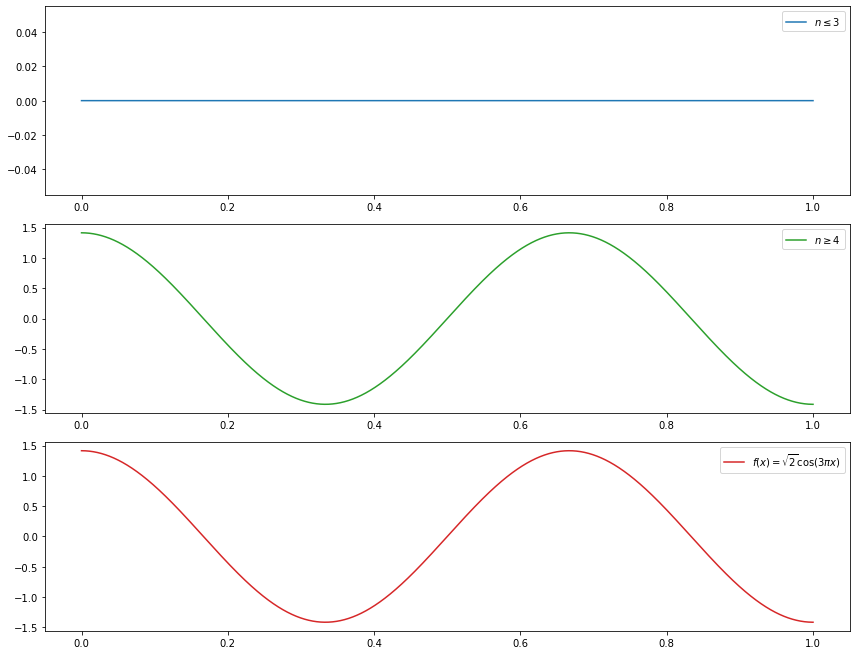
\includegraphics{Figure-22-06}
\end{figure}

\textbf{(b)} can be solved with the definition of \(\beta_{j}\):
For \(j = 1\),
\[
\beta_{j} = \langle f, \phi_{1} \rangle = \int_{0}^{1} f(x) \phi_{1}(x) dx = \int_{0}^{1} \sin(\pi x) dx = \frac{2}{\pi}
\]
For \(j \geq 2\),
\[
\beta_{j} = \langle f, \phi_{j} \rangle = \int_{0}^{1} f(x) \phi_{j}(x) dx = \int_{0}^{1} \sin(\pi x) \left( \sqrt{2} \cos((j-1) \pi x) \right) dx = \frac{\sqrt{2} (\cos(\pi j) - 1)}{\pi j^{2} - 2 \pi j }
\]
so
\[
\beta_{j} = \begin{cases}
\frac{2}{\pi} & \text{if } j = 1\\
-\frac{2\sqrt{2}}{\pi j^{2} - 2 \pi j} & \text{if } j \text{ is odd}, j > 1 \\
0 & \text{if } j \text{ is even}
\end{cases}
\]

\begin{python}
import numpy as np
def beta_{j}(j):
    if j % 2 == 0:
        return 0
    if j == 1:
        return 2 / np.pi
    return -np.sqrt(2)*2 / ((np.pi * j * j) - (2 * np.pi * j))
def phi_{j}(j):
    def f(x):
        if j == 1:
            return np.ones_like(x)
        return np.sqrt(2) * np.cos((j - 1) * np.pi * x)
    return f
def partial_sum(n, x):
    lx = len(x)
    terms = np.empty((n, lx))
    for j in range(1, n + 1):
        terms[j - 1] = beta_{j}(j) * phi_{j}(j)(xx)
    return terms.sum(axis = 0)
\end{python}

\begin{python}
# Plot in separate boxes for ease of visualization
import matplotlib.pyplot as plt
%matplotlib inline
step = 1e-4
xx = np.arange(0, 1 + step, step=step)
plt.figure(figsize=(12, 12))
def do_subplot(index, xx, yy, label, color):
    ax = plt.subplot(4, 1, index)
    ax.plot(xx, yy, label=label, color=color)
    ax.legend()    
do_subplot(1, xx, partial_sum(4,  xx), label=r'$n = %i$' % 4, color='C0')
do_subplot(2, xx, partial_sum(8,  xx), label=r'$n = %i$' % 8, color='C1')
do_subplot(3, xx, partial_sum(16, xx), label=r'$n = %i$' % 16, color='C2')
do_subplot(4, xx, np.sin(np.pi * xx), label=r'$f(x) = \sin(\pi x)$', color='C3')
    
plt.tight_layout()
plt.legend()
plt.show()
\end{python}

\begin{figure}[H]
\centering
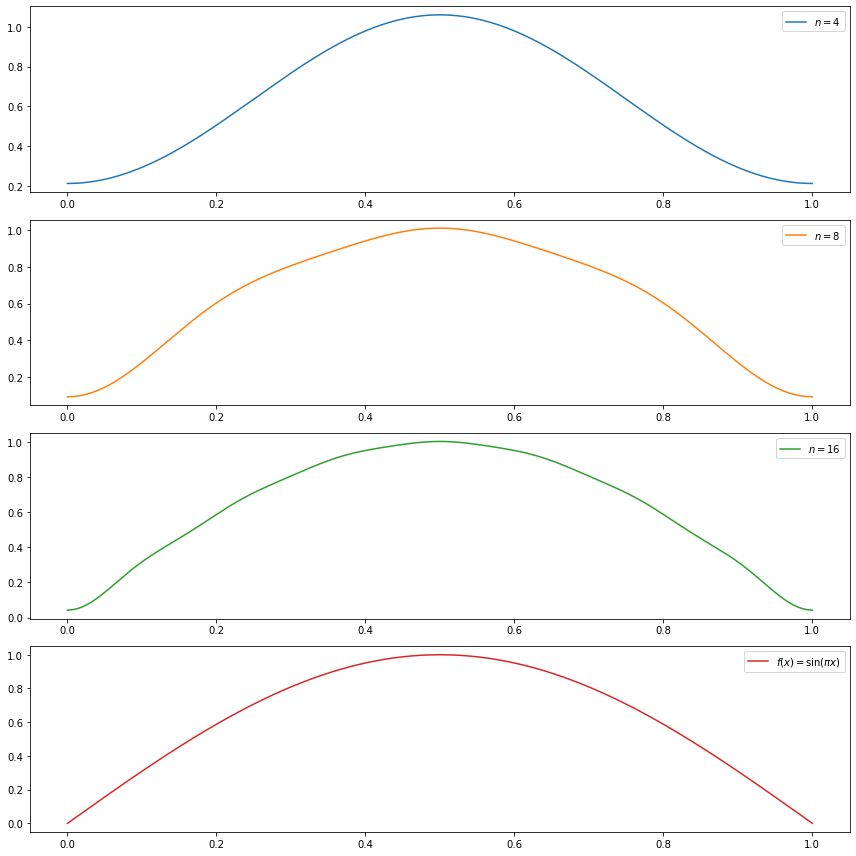
\includegraphics{Figure-22-07}
\end{figure}

\textbf{(c)}

\begin{python}
import numpy as np
T = np.array([.1, .13, .15, .23, .25, .40, .44, .65, .76, .78, .81])
H = np.array([4, -5, 3, -4, 5, -4.2, 2.1, 4.3, -3.1, 2.1, -4.2])
def phi_{j}(j):
    def f(x):
        if j == 1:
            return np.ones_like(x)
        return np.sqrt(2) * np.cos((j - 1) * np.pi * x)
    return f
def f(x):
    def K(t):
        return (1 + np.sign(t))/2
    return (H.reshape(1, -1) * K(
        x.reshape(-1, 1).repeat(len(T), axis=1) - T.reshape(-1, 1).repeat(len(x), axis=1).T)
    ).sum(axis = 1)
\end{python}

\begin{python}
N = 10000
step = 1 / N
xx = np.arange(0, 1 + step, step=step)
J = 256
estimated_beta = np.empty(J)
for j in range(1, J + 1):
    estimated_beta[j - 1] = f(xx) @ phi_{j}(j)(xx) / N
    
def beta_{j}(j):
    return estimated_beta[j - 1]
def partial_sum(n, x):
    lx = len(x)
    terms = np.empty((n, lx))
    for j in range(1, n + 1):
        terms[j - 1] = beta_{j}(j) * phi_{j}(j)(xx)
    return terms.sum(axis = 0)
\end{python}

\begin{python}
# Plot in separate boxes for ease of visualization
import matplotlib.pyplot as plt
%matplotlib inline
step = 1e-4
xx = np.arange(0, 1 + step, step=step)
plt.figure(figsize=(12, 12))
def do_subplot(index, xx, yy, label, color):
    ax = plt.subplot(4, 1, index)
    ax.plot(xx, yy, label=label, color=color)
    ax.legend()    
do_subplot(1, xx, partial_sum(16,  xx), label=r'$n = %i$' % 16, color='C0')
do_subplot(2, xx, partial_sum(64,  xx), label=r'$n = %i$' % 64, color='C1')
do_subplot(3, xx, partial_sum(256, xx), label=r'$n = %i$' % 256, color='C2')
do_subplot(4, xx, f(xx), label=r'$f(x) = \sum_{j} h_{j} K(x - t_{j}) $', color='C3')
    
plt.tight_layout()
plt.legend()
plt.show()
\end{python}

\begin{figure}[H]
\centering
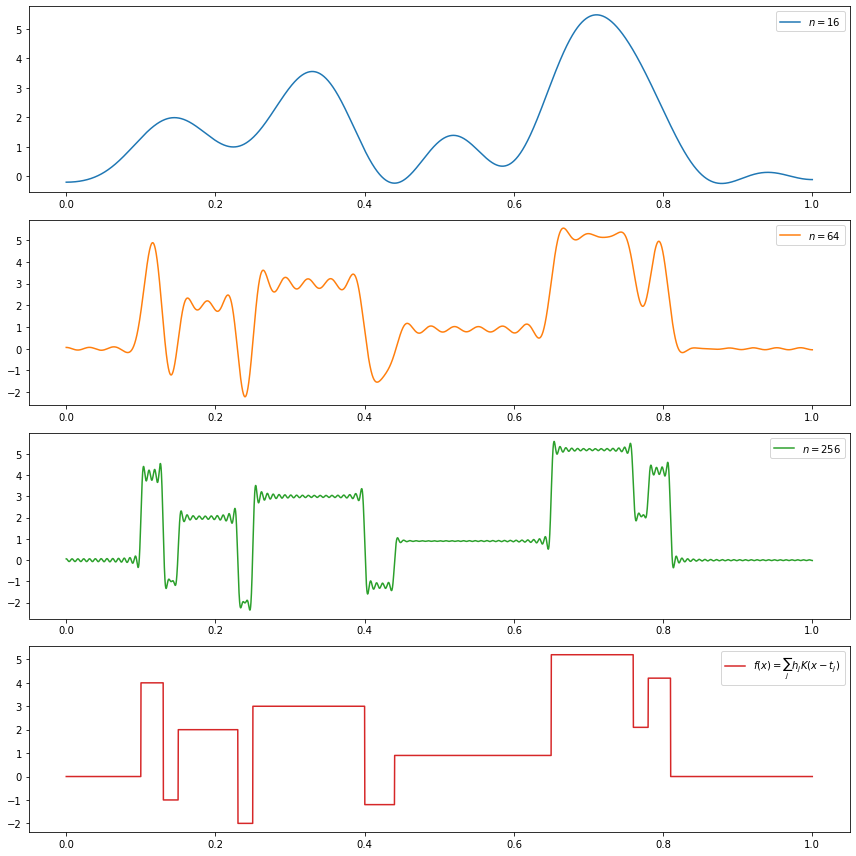
\includegraphics{Figure-22-08}
\end{figure}

\textbf{(d)}

\begin{python}
import numpy as np
def phi_{j}(j):
    def f(x):
        if j == 1:
            return np.ones_like(x)
        return np.sqrt(2) * np.cos((j - 1) * np.pi * x)
    return f
def f(x):
    return np.sqrt(x * (1 - x)) * np.sin(2.1 * np.pi / (x + 0.05))
\end{python}

\begin{python}
N = 10000
step = 1 / N
xx = np.arange(0, 1 + step, step=step)
J = 512
estimated_beta = np.empty(J)
for j in range(1, J + 1):
    estimated_beta[j - 1] = f(xx) @ phi_{j}(j)(xx) / N
    
def beta_{j}(j):
    return estimated_beta[j - 1]
def partial_sum(n, x):
    lx = len(x)
    terms = np.empty((n, lx))
    for j in range(1, n + 1):
        terms[j - 1] = beta_{j}(j) * phi_{j}(j)(xx)
    return terms.sum(axis = 0)
\end{python}

\begin{python}
# Plot in separate boxes for ease of visualization
import matplotlib.pyplot as plt
%matplotlib inline
step = 1e-4
xx = np.arange(0, 1 + step, step=step)
plt.figure(figsize=(12, 12))
def do_subplot(index, xx, yy, label, color):
    ax = plt.subplot(4, 1, index)
    ax.plot(xx, yy, label=label, color=color)
    ax.legend()    
do_subplot(1, xx, partial_sum(16,  xx), label=r'$n = %i$' % 16, color='C0')
do_subplot(2, xx, partial_sum(64,  xx), label=r'$n = %i$' % 64, color='C1')
do_subplot(3, xx, partial_sum(512, xx), label=r'$n = %i$' % 512, color='C2')
do_subplot(4, xx, f(xx), label=r'$f(x) = \sqrt{x (1 - x)} \sin \left( \frac{2.1 \pi}{(x + .05)} \right)$', color='C3')
    
plt.tight_layout()
plt.legend()
plt.show()
\end{python}

\begin{figure}[H]
\centering
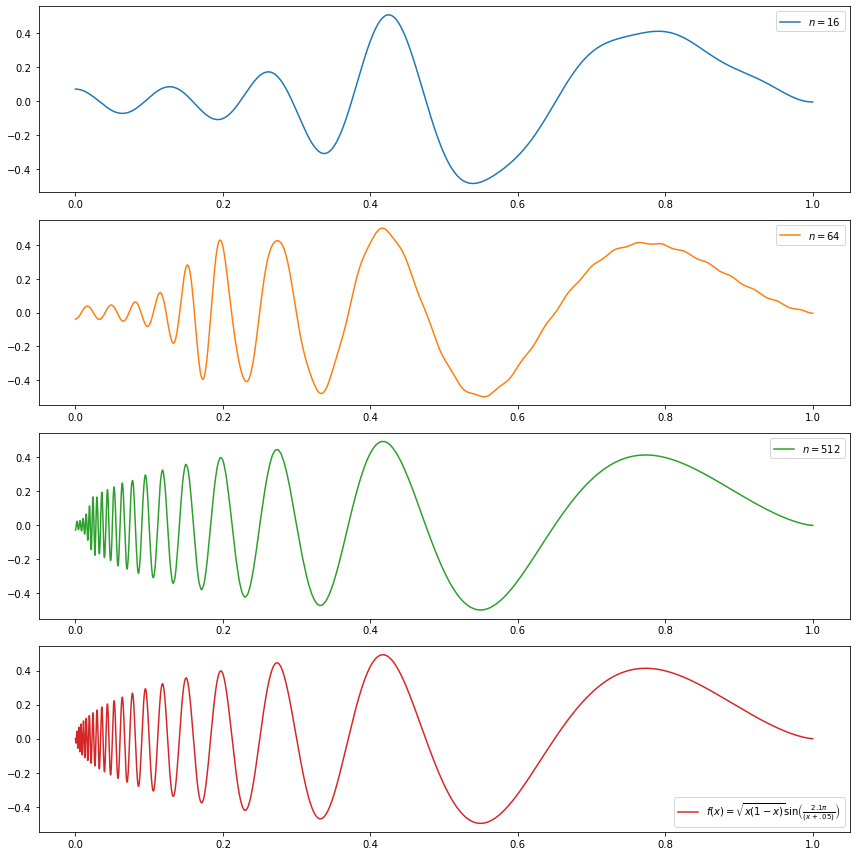
\includegraphics{Figure-22-09}
\end{figure}


\textbf{Exercise 22.6.7}. Consider the glass fragments data. Let \(Y\)
be the refractive index and let \(X\) be aluminium content (the fourth
variable).
\textbf{(a)} Do a nonparametric regression to fit the model
\(Y = f(x) + \epsilon\) using the cosine basis method. The data are not
on a regular grid. Ignore this when estimating the function. (But do
sort the data first.) Provide a function estimate, an estimate of the
risk, and a confidence band.
\textbf{(b)} Use the wavelet method to estimate \(f\).

\textbf{Solution}.

\begin{python}
import numpy as np
import pandas as pd
data = pd.read_csv('data/glass.txt', delim_whitespace=True)
data = data[['Al', 'RI']].sort_values(by='Al', ignore_{i}ndex=True)
X, Y = data['Al'], data['RI']
\end{python}
\textbf{(a)}
\textbf{Orthogonal Series Regression Estimator}
\begin{enumerate}[tightlist,label={\arabic*.}]
\item
  Let
\end{enumerate}
\[
\hat{\beta}_{j} = \frac{1}{n} \sum_{i=1}^{n} Y_{i} \phi_{i}(x_{i}), \quad j = 1, \dots, n
\]
\begin{enumerate}[tightlist,label={\arabic*.}]
\item
  Let
\end{enumerate}
\[
\hat{\sigma}^{2} = \frac{n}{k} \sum_{i=n-k+1}^{n} \hat{\beta}_{j}^{2}
\]
where \(k \approx n / 4\).
\begin{enumerate}[tightlist,label={\arabic*.},resume]
\item
  For \(1 \leq J \leq n\), compute the risk estimate
\end{enumerate}
\[
\hat{R}(J) = J \frac{\hat{\sigma}^{2}}{n} + \sum_{j=J+1}^{n} \left(\hat{\beta}_{j}^{2} - \frac{\hat{\sigma}^{2}}{n} \right)_{+}
\]
\begin{enumerate}
\def\labelenumi{\arabic{enumi}.}
\setcounter{enumi}{3}
\item
  Choose \(\hat{J} \in \{1, \dots, n \}\) to minimize \(\hat{R}(J)\).
\item
  Let
\end{enumerate}
\[
\hat{f}(x) = \sum_{j=1}^J \hat{\beta}_{j} \phi_{j}(x)
\]

\textbf{Theorem 22.11}. Suppose the estimate \(\hat{r}\) is based on
\(J\) terms and $\hat{\sigma}^{2} = \frac{n}{k} \sum\_\{i=n-k+1\}^{n}
\hat{\beta}\_{j}^{2} $. Assume that \(J < n - k + 1\). An approximate
\(1 - \alpha\) confidence band for \(\bar{r}\) is \((\ell, u)\),
where
\[
\ell(x) = \hat{r}(x) - K \sqrt{J} \sqrt{\frac{z_{\alpha} \hat{\tau}}{\sqrt{n}} + \frac{J \hat{\sigma}^{2}}{n}}
\quad \text{and} \quad u(x) = \hat{r}(x) + K \sqrt{J} \sqrt{\frac{z_{\alpha} \hat{\tau}}{\sqrt{n}} + \frac{J \hat{\sigma}^{2}}{n}}
\]
where
\[
K = \max_{1 \leq j \leq J} \max_x | \phi_{j}(x) |
\]
and
\[
\hat{\tau}^{2} = \frac{2 J \hat{\sigma}^{4}}{n} \left( 1 + \frac{J}{k} \right)
\]
and \(k = n / 4\) as used in the definition of \(\hat{\sigma}^{2}\). In
the cosine basis, \(K = \sqrt{2}\).

\begin{python}
# Cosine basis function
def phi_{j}(j):
    def f(x):
        if j == 1:
            return np.ones_like(x)
        return np.sqrt(2) * np.cos((j - 1) * np.pi * x)
    return f
\end{python}

\begin{python}
from scipy.stats import norm
def estimate_r(X, Y, alpha=0.05):
    n = len(X)
    # Rescale from [X.min(), X.max()] to [0, 1]
    def X_to_L2(t):
        return (t - X.min()) / (X.max() - X.min())
    
    X_scaled = X_to_L2(X)
    beta_hat = np.empty(n)
    for j in range(1, n+1):
        beta_hat[j - 1] = np.sum(Y @ phi_{j}(j)(X_scaled)) / n
        
    k = int(np.ceil(n / 4))
    sigma2_hat = np.sum(beta_hat[-k:]**2) * (n / k)
    risk_hat = np.zeros(n)
    for J in range(1, n + 1):
        risk_hat[J - 1] = J * sigma2_hat/n 
                          + np.sum(np.maximum(beta_hat[J:]**2 
                          - sigma2_hat/n, 0))
    def r_hat(x):
        xx = X_to_L2(x)
        result = np.zeros_like(xx)
        for j in range(1, J_hat):
            result += beta_hat[j - 1] * phi_{j}(j)(xx)
        return result
        
    J_hat = np.argmin(risk_hat) + 2
    tau_hat = sigma2_hat * np.sqrt((2 * J_hat / n) * (1 + J_hat / k))
    z_alpha = norm.ppf(1 - alpha / 2)
    c = np.sqrt(2 * J * ((z_alpha * tau_hat / np.sqrt(n)) + (J_hat * sigma2_hat / n)))
    
    def r_lower(x):
        return r_hat(x) - c
    
    def r_upper(x):
        return r_hat(x) + c
            
    return r_hat, r_lower, r_upper
\end{python}

\begin{python}
r_hat, r_lower, r_upper = estimate_r(X, Y, alpha=0.05)
\end{python}

\begin{python}
import matplotlib.pyplot as plt
plt.figure(figsize=(12, 8))
plt.scatter(X, Y, color='C0', marker='x', label='Data')
X_min, X_max = X.min(), X.max()
t = np.arange(X_min, X_max, step=(X_max - X_min) / 1000)
plt.plot(t, r_hat(t), color='purple', label='$\hat{r}(x)$')
plt.plot(t, r_lower(t), color='red', alpha=0.5, label='95% lower bound')
plt.plot(t, r_upper(t), color='green', alpha=0.5, label='95% upper bound')
plt.xlabel('Al content')
plt.ylabel('Refractive Index')
plt.legend()
plt.show()
\end{python}

\begin{figure}[H]
\centering
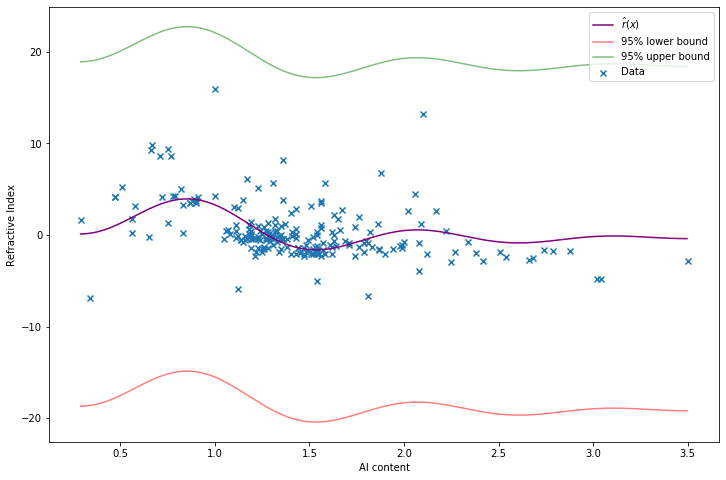
\includegraphics{Figure-22-10}
\end{figure}

\textbf{(b)}
\textbf{Haar Wavelet Regression}
\begin{enumerate}[tightlist,label={\arabic*.}]
\item
  Let \(J = \log_{2} n\) and define
\end{enumerate}
\[
\hat{\alpha} = \frac{1}{n} \sum_{i} \phi(x_{i}) Y_{i}
\quad \text{and} \quad
D_{j, k} = \frac{1}{n} \sum_{i} \psi_{j, k}(x_{i}) Y_{i}
\]
for \(0 \leq j \leq J - 1\)
\begin{enumerate}[tightlist,label={\arabic*.}]
\item
  Estimate \(\sigma\) by
\end{enumerate}
\[
\hat{\sigma} = \sqrt{n} \; \times \; \frac{\text{median} \left( \left| D_{J-1, k} : k = 0, \dots, 2^{J - 1} - 1\right| \right)}{0.6745}
\]
\begin{enumerate}[tightlist,label={\arabic*.},resume]
\item
  Apply universal thresholding:
\end{enumerate}
\[
\hat{\beta}_{j, k} = \begin{cases}
D_{j, k} & \text{if } \left| D_{j, k} \right| > \hat{\sigma} \sqrt{\frac{2 \log n}{n}} \\
0 & \text{otherwise}
\end{cases}
\]
\begin{enumerate}[tightlist,label={\arabic*.},resume]
\item
  Set
\end{enumerate}
\[
\hat{f}(x) = \hat{\alpha} \phi(x) + \sum_{j = j_{0}}^{J - 1} \sum_{k = 0}^{2^{j} - 1} \hat{\beta}_{j, k} \psi_{j, k}(x)
\]

\begin{python}
# Wavelet base functions
import numpy as np
def haar_father_wavelet(x):
    return np.where((x >= 0) & (x < 1), 1, 0)
def haar_mother_wavelet(x):
    return np.where((x >= 0) & (x < 1),  np.where(x <= 1/2, -1, 1), 0)
def psi_wavelet(j, k):
    def f(x):
        return 2**(j / 2) * haar_mother_wavelet((2**j)*x - k)
    return f
\end{python}

\begin{python}
def estimate_r(X, Y):
    n = len(Y)
    J = int(np.ceil(np.log2(n)))
    def X_to_L2(t):
        return (t - X.min()) / (X.max() - X.min())
    xx = X_to_L2(X)
    alpha_hat = np.sum(Y) / n
    D = {}
    for j in range(J):
        D[j] = np.zeros(2**j)
        for k in range(2**j):
            D[j][k] = psi_wavelet(j, k)(xx) @ Y / n
    sigma_hat = np.sqrt(n) * np.median(np.abs(D[J - 1])) / 0.6745
    threshold = sigma_hat * np.sqrt(2 * np.log(n) / n)
    beta_hat = [(j, k, v) for j, values in D.items() for k, v in enumerate(values) \
        if np.abs(v) > threshold]
    def r_hat(X):
        xx = X_to_L2(X)
        return alpha_hat * haar_father_wavelet(xx) \
            + np.sum(np.array([v * psi_wavelet(j, k)(xx) for j, k, v in beta_hat]), axis=0)
    
    return r_hat
\end{python}

\begin{python}
r_hat = estimate_r(X, Y)
\end{python}

\begin{python}
import matplotlib.pyplot as plt
%matplotlib inline
plt.figure(figsize=(12, 8))
plt.scatter(X, Y, color='C0', marker='x', label='Data')
X_min, X_max = X.min(), X.max()
t = np.arange(X_min, X_max, step=(X_max - X_min) / 10000)
plt.plot(t, r_hat(t), color='purple', label='$\hat{r}(x)$')
plt.xlabel('Al content')
plt.ylabel('Refractive Index')
plt.legend()
plt.show()
\end{python}

\begin{figure}[H]
\centering
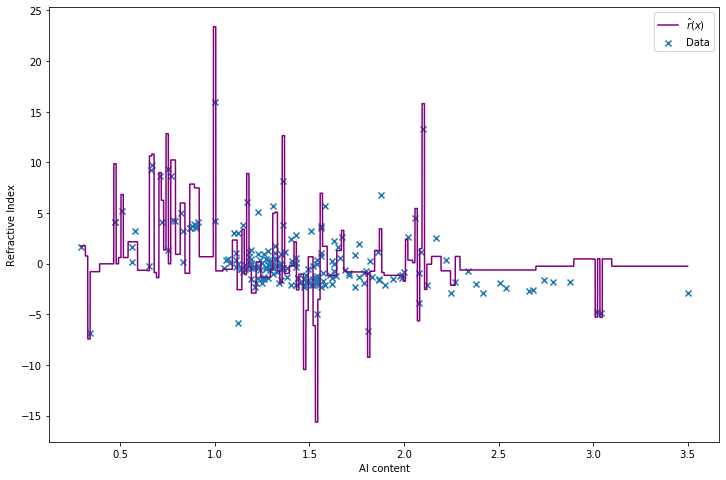
\includegraphics{Figure-22-11}
\end{figure}


\textbf{Exercise 22.6.8}. Show that the Haar wavelets are orthonormal.

\textbf{Solution}.
Recalling the definitions:
The \textbf{father Haar wavelet} of \textbf{Haar scaling function} is
defined by
\[
\phi(x) = \begin{cases}
1 & \text{if } 0 \leq x < 1 \\
0 & \text{otherwise}
\end{cases}
\]
The \textbf{mother Haar wavelet} is defined by
\[
\psi(x) = \begin{cases}
-1 & \text{if } 0 \leq x \leq \frac{1}{2} \\
1  & \text{if } \frac{1}{2} < x \leq 1
\end{cases}
\]
For any integers \(j\) and \(k\) define
\[
\phi_{j, k}(x) = 2^{j/2} \phi(2^{j} x - k) 
\quad \text{and} \quad
\psi_{j, k}(x) = 2^{j/2} \psi(2^{j} x - k)
\]
The function \(\psi_{j, k}\) has the same shape as \(\psi\) but it has
been rescaled by a factor of \(2^{j/2}\) and shifted by a factor of
\(k\).
Let
\[
W_{j} = \{\psi_{j, k}, \; k = 0, 1, \dots, 2^{j} - 1\}
\]
be the set of rescaled and shifted mother wavelets at resolution \(j\).

\textbf{Theorem 22.13}. The set of functions
\[
\left\{ \phi, W_{0}, W_{1}, W_{2}, \dots \right\}
\]
is an orthonormal basis for \(L_{2}(0, 1)\).
\textbf{Proof}.
Normality:
\begin{align*}
\langle \phi, \phi \rangle &= \int_{0}^{1} \phi^{2}(x) dx = \int_{0}^{1} 1 \; dx = 1 \\
\langle \psi_{j, k}, \psi_{j, k} \rangle &= \int_{0}^{1} \psi_{j, k}^{2}(x) dx \\
&= \int_{0}^{1} \left( 2^{j / 2} \psi(2^{j} x - k) \right)^{2} dx \\
&= \int_{-k}^{2^{j} - k} 2^{j}  \psi^{2}(y) \left( 2^{-j} dy \right) \\
&= \int_{0}^{1} 1 \; dy = 1
\end{align*}
Orthogonality:
\begin{align*}
\langle \phi, \psi_{j, k} \rangle &= \int_{0}^{1} \phi(x) \psi_{j, k}(x) dx \\
&= \int_{0}^{1}  2^{j / 2} \psi(2^{j} x - k) dx  \\
&= \int_{-k}^{2^{j} - k} 2^{j / 2}  \psi(y) \left( 2^{-j} dy \right) \\
&= 2^{-j/2} \int_{0}^{1} \psi(y) dy = 1
\end{align*}
since \(\psi(y)\) has values \(-1\) for \(y \in [0, 1/2]\) and \(1\) for
\([1/2, 1]\), and 0 otherwise, and \([0, 1] \subset [-k, 2^{j} - k]\).
\begin{align*}
\langle \psi_{a, b}, \psi_{c, d} \rangle &= \int_{0}^{1} \psi_{a, b}(x) \psi_{c, d}(x)
\end{align*}
For each wavelet \(\psi_{j, k}\), consider the domain of values that
produce a non-zero function output,
\[
F_{j, k} = \{ x : \psi_{j, k}(x) \neq 0 \} = \left[\frac{k}{2^{j}}, \frac{k + 1}{2^{j}} \right]
\]
Also consider the regions that produce +1 and -1 outputs,
\[
F_{j, k}^+ = \{ x : \psi_{j, k}(x) = 1 \} = \left[\frac{k + \frac{1}{2}}{2^{j}}, \frac{k + 1}{2^{j}} \right]
\quad \text{and} \quad
F_{j, k}^- = \{ x : \psi_{j, k}(x) = 1 \} = \left[\frac{k}{2^{j}}, \frac{k + \frac{1}{2}}{2^{j}} \right]
\]
If \(a = c\), \(b \neq d\), then the non-zero domain of the wavelets do
not overlap -- each increment or decrement in the second parameter
`shifts' the whole non-zero domain by its size, i.e.~the diameter of
\(F_{j, k}\) which is \(2^{-j}\). Therefore, in this case, the integral
is zero.
If \(a \neq c\), assuming without loss of generality \(a < c\), then we
may have intersection in the non-zero areas. But in that case, the
non-zero domain is fully contained within the plus or minus domain,
\(F_{c, d} \subset F_{a, b}^+\) or \(F_{c, d} \subset F_{a, b}^-\).
Therefore, in this case, the integral must also be zero.
Since we covered all cases, we have shown orthogonality. Since we have
orthogonality and normality, the basis is orthonormal, proving the
Theorem.

\textbf{Exercise 22.6.9}. Consider again the doppler signal:
\[
f(x) = \sqrt{x (1 - x)} \sin \left( \frac{2.1 \pi}{x + 0.05} \right)
\]
Let \(n = 1024\) and let \((x_{1}, \dots, x_{n}) = (1/n, \dots, 1)\).
Generate data
\[
Y_{i} = f(x_{i}) + \sigma \epsilon_{i}
\]
where \(\epsilon_{i} \sim N(0, 1)\).
\textbf{(a)} Fit the curve using the cosine basis method. Plot the
function estimate and confidence band for \(J = 10, 20, \dots, 100\).
\textbf{(b)} Use Haar wavelets to fit the curve.

\textbf{Solution}. Pick \(\sigma = 0.1\) when generating the data:

\begin{python}
import numpy as np
from scipy.stats import norm
def f(x):
    return np.sqrt(x * (1 - x)) * np.sin( (2.1 * np.pi) / (x + 0.05) )
n = 1024
sigma = 0.1
X = np.arange(1, n + 1) / n
Y = f(X) + norm.rvs(loc=0, scale=sigma, size=n)
\end{python}

\begin{python}
import matplotlib.pyplot as plt
%matplotlib inline
plt.figure(figsize=(12, 8))
plt.scatter(X, Y, marker='x')
plt.show()
\end{python}

\begin{figure}[H]
\centering
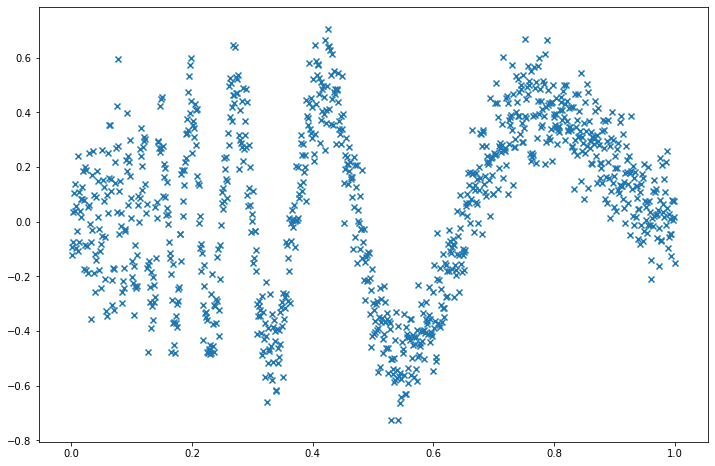
\includegraphics{Figure-22-12}
\end{figure}

\textbf{(a)}

\begin{python}
# Cosine basis function
def phi_{j}(j):
    def f(x):
        if j == 1:
            return np.ones_like(x)
        return np.sqrt(2) * np.cos((j - 1) * np.pi * x)
    return f
\end{python}

\begin{python}
from scipy.stats import norm
def estimate_r(X, Y, J=None, alpha=0.05):
    n = len(X)
    # Rescale from [X.min(), X.max()] to [0, 1]
    def X_to_L2(t):
        return (t - X.min()) / (X.max() - X.min())
    
    X_scaled = X_to_L2(X)
    beta_hat = np.empty(n)
    for j in range(1, n+1):
        beta_hat[j - 1] = np.sum(Y @ phi_{j}(j)(X_scaled)) / n
        
    k = int(np.ceil(n / 4))
    sigma2_hat = np.sum(beta_hat[-k:]**2) * (n / k)
    if J is None:
        # J not specified, pick J that minimizes risk
        risk_hat = np.zeros(n)
        for J in range(1, n + 1):
            risk_hat[J - 1] = J * sigma2_hat/n + np.sum(np.maximum(beta_hat[J:]**2 
                - sigma2_hat/n, 0))
        J_hat = np.argmin(risk_hat) + 2
    else:
        # Use pre-specified J
        assert J <= n, "J must be smaller than n"
        J_hat = J
    def r_hat(x):
        xx = X_to_L2(x)
        result = np.zeros_like(xx)
        for j in range(1, J_hat):
            result += beta_hat[j - 1] * phi_{j}(j)(xx)
        return result
        
    tau_hat = sigma2_hat * np.sqrt((2 * J_hat / n) * (1 + J_hat / k))
    z_alpha = norm.ppf(1 - alpha / 2)
    c = np.sqrt(2 * J * ((z_alpha * tau_hat / np.sqrt(n)) + (J_hat * sigma2_hat / n)))
    
    def r_lower(x):
        return r_hat(x) - c
    
    def r_upper(x):
        return r_hat(x) + c
            
    return r_hat, r_lower, r_upper, J_hat
\end{python}

\begin{python}
import matplotlib.pyplot as plt
def do_subplot(i, J):
    ax = plt.subplot(5, 2, i)
    r_hat, r_lower, r_upper, J_hat = estimate_r(X, Y, J=J)
    ax.scatter(X, Y, color='C0', marker='x', alpha=0.5, label='Data')
    ax.plot(X, r_hat(X), color='purple', label='$r(x)$')
    ax.plot(X, r_lower(X), color='red', alpha=0.5, label='95% lower bound')
    ax.plot(X, r_upper(X), color='green', alpha=0.5, label='95% upper bound')
    ax.set_title('J = %i' % J)
    
plt.figure(figsize=(12, 12))
for i, J in enumerate([10, 20, 30, 40, 50, 60, 70, 80, 90, 100]):
    
    do_subplot(i + 1, J)
plt.tight_layout()
plt.show()
plt.figure(figsize=(14.5, 8))
r_hat, r_lower, r_upper, J_hat = estimate_r(X, Y, J=None)
plt.scatter(X, Y, color='C0', marker='x', alpha=0.5, label='Data')
plt.plot(X, r_hat(X), color='purple', label='$r(x)$')
plt.plot(X, r_lower(X), color='red', alpha=0.5, label='95% lower bound')
plt.plot(X, r_upper(X), color='green', alpha=0.5, label='95% upper bound')
plt.title('J = %i (min risk)' % J_hat)
plt.show()
\end{python}

\begin{figure}[H]
\centering
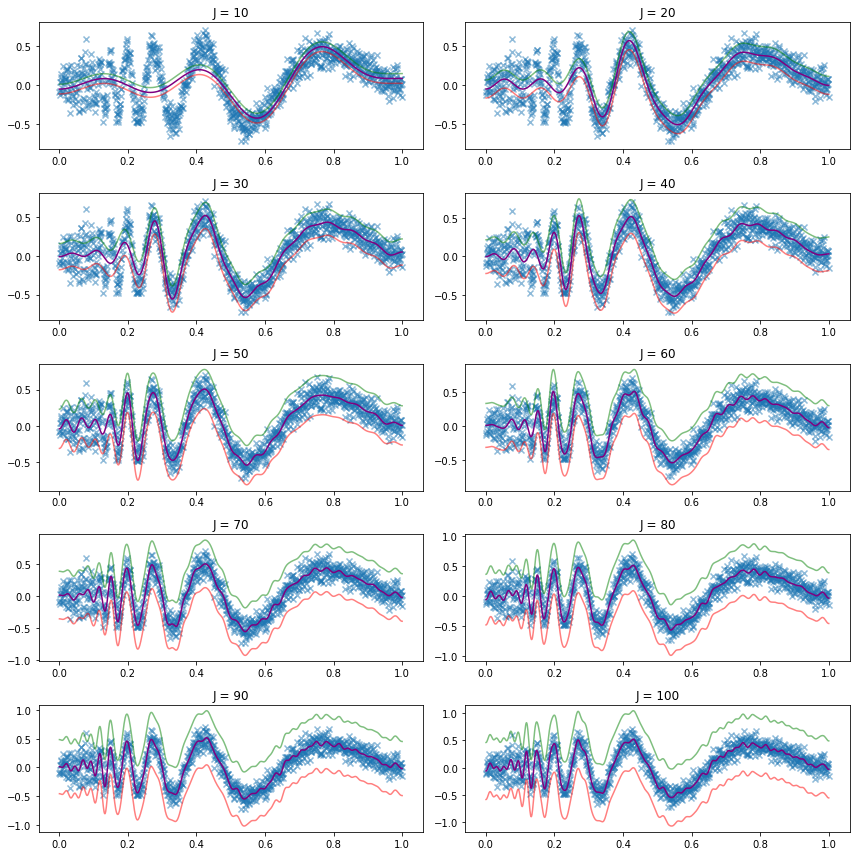
\includegraphics{Figure-22-13}
\end{figure}

\begin{figure}[H]
\centering
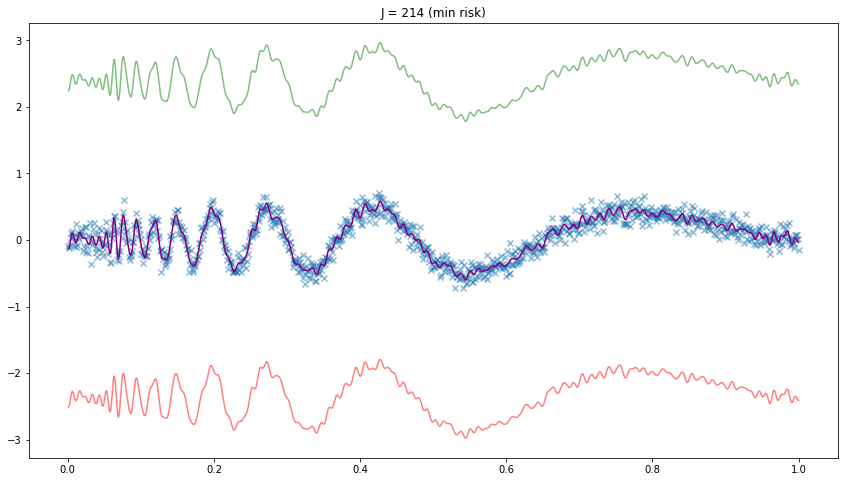
\includegraphics{Figure-22-14}
\end{figure}

\textbf{(b)}

\begin{python}
# Wavelet base functions
import numpy as np
def haar_father_wavelet(x):
    return np.where((x >= 0) & (x < 1), 1, 0)
def haar_mother_wavelet(x):
    return np.where((x >= 0) & (x < 1),  np.where(x <= 1/2, -1, 1), 0)
def psi_wavelet(j, k):
    def f(x):
        return 2**(j / 2) * haar_mother_wavelet((2**j)*x - k)
    return f
\end{python}

\begin{python}
def estimate_r(X, Y):
    n = len(Y)
    J = int(np.ceil(np.log2(n)))
    def X_to_L2(t):
        return (t - X.min()) / (X.max() - X.min())
    xx = X_to_L2(X)
    alpha_hat = np.sum(Y) / n
    D = {}
    for j in range(J):
        D[j] = np.zeros(2**j)
        for k in range(2**j):
            D[j][k] = psi_wavelet(j, k)(xx) @ Y / n
    sigma_hat = np.sqrt(n) * np.median(np.abs(D[J - 1])) / 0.6745
    threshold = sigma_hat * np.sqrt(2 * np.log(n) / n)
    beta_hat = [(j, k, v) for j, values in D.items() for k, v in enumerate(values) \ 
        if np.abs(v) > threshold]
    def r_hat(X):
        xx = X_to_L2(X)
        return alpha_hat * haar_father_wavelet(xx) \
            + np.sum(np.array([v * psi_wavelet(j, k)(xx) for j, k, v in beta_hat]), axis=0)
    
    return r_hat
\end{python}

\begin{python}
r_hat = estimate_r(X, Y)
\end{python}

\begin{python}
import matplotlib.pyplot as plt
plt.figure(figsize=(12, 8))
plt.scatter(X, Y, color='C0', alpha=0.5, marker='x', label='Data')
X_min, X_max = X.min(), X.max()
t = np.arange(X_min, X_max, step=(X_max - X_min) / 10000)
plt.plot(t, r_hat(t), color='purple', label='$\hat{r}(x)$')
plt.legend()
plt.show()
\end{python}

\begin{figure}[H]
\centering
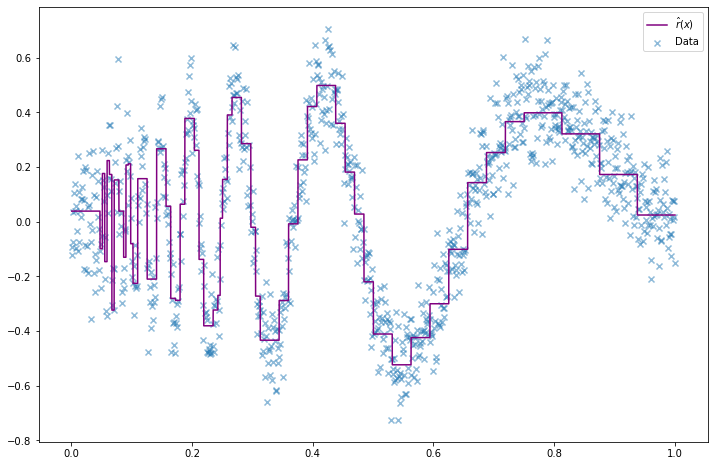
\includegraphics{Figure-22-15}
\end{figure}


\textbf{Exercise 22.6.10 (Haar density estimation)}. Let
\(X_{1}, \dots, X_{n} \sim f\) for some density \(f\) on \([0, 1]\).
Consider constructing a wavelet histogram. Let \(\phi\) and \(\psi\) be
the Haar father and mother wavelet. Write
\[
f(x) \approx \phi(x) + \sum_{j=0}^{J - 1} \sum_{k=0}^{2^{j} - 1} \beta_{j, k} \psi_{j, k}(x)
\]
where \(J \approx \log_{2}(n)\). Let
\[
\hat{\beta}_{j, k} = \frac{1}{n} \sum_{i=1}^{n} \psi_{j, k}(X_{i})
\].
\textbf{(a)} Show that \(\hat{\beta}_{j, k}\) is an unbiased estimate of
\(\beta_{j, k}\).
\textbf{(b)} Define the Haar histogram
\[
\hat{f}(x) = \phi(x) + \sum_{j=0}^{B} \sum_{k=0}^{2^{j} - 1} \hat{\beta}_{j, k} \psi_{j, k}(x)
\]
for \(0 \leq B \leq J - 1\).
\textbf{(c)} Find an approximate expression for the MSE as a function of
\(B\).
\textbf{(d)} Generate \(n = 1000\) observations from a
\(\text{Beta}(15, 4)\) density. Estimate the density using the Haar
histogram. Use leave-one-out cross validation to choose \(B\).

\textbf{Solution}.
\textbf{(a)}
\[
\EXP(\hat{\beta}_{j, k}) = \frac{1}{n} \sum_{i=1}^{n} \EXP(\psi_{j, k}(X_{i}))
= \EXP(\psi_{j, k}(X_{1})) = \int_{0}^{1} \psi_{j, k}(x) dx = \beta_{j, k}
\]
\textbf{(b)} Interpret ``define'' as ``implement''.

\begin{python}
# Wavelet base functions
import numpy as np
def haar_father_wavelet(x):
    return np.where((x >= 0) & (x < 1), 1, 0)
def haar_mother_wavelet(x):
    return np.where((x >= 0) & (x < 1),  np.where(x <= 1/2, -1, 1), 0)
def psi_wavelet(j, k):
    def f(x):
        return 2**(j / 2) * haar_mother_wavelet((2**j)*x - k)
    return f
\end{python}

\begin{python}
import numpy as np
def haar_histogram(X, B): 
    n = len(X)
    
    def X_to_L2(t):
        return (t - X.min()) / (X.max() - X.min())
    
    xx = X_to_L2(X)
    D = {}
    for j in range(B):
        D[j] = np.zeros(2**j)
        for k in range(2**j):
            D[j][k] = np.sum(psi_wavelet(j, k)(xx)) / n
            
    # No thresholding
    beta_hat = [(j, k, v) for j, values in D.items() for k, v in enumerate(values)]
    
    def f_hat(x):
        xx = X_to_L2(x)
        return haar_father_wavelet(xx) \
            + np.sum(np.array([v * psi_wavelet(j, k)(xx) for j, k, v in beta_hat]), axis=0)
    
    return f_hat
\end{python}
\textbf{(c)} The orthonormal basis of Haar wavelets has its functions
ordered as
\[
\begin{array}{ccc}
\phi, \\
\psi_{0, 0}, \\
\psi_{1, 0}, & \psi_{1, 1}, \\
\psi_{2, 0}, & \dots, & \psi_{2, 2}, \\
\vdots \\
\psi_{j, 0}, & \dots, & \psi_{j, 2^{k} - 1}, \\
\vdots
\end{array}
\]
where each row of wavelets other than the first goes from
\(\psi_{j, 0}\) to \(\psi_{j, 2^{j} - 1}\), containing \(2^{j}\) functions.
We can label them in order
\[
q_{1}, q_{2}, \dots 
\quad \text{where }q_{n} = \begin{cases}
\phi & \text{if }  n = 1 \\
\psi_{\lceil \log_{2} n \rceil- 1, n + 1 - \lceil \log_{2} n \rceil } & \text{otherwise}
\end{cases}
\]
Now, limiting the Haar histogram estimator to hyperparameter \(B\) is
equivalent to limiting it to only use the first \(2^{B + 1}\) functions.
Then, we can use Theorem 22.5 to calculate the risk on the basis of the
\(q_{j}\)s, where \(J = 2^{B + 1}\):
\[
R = \sum_{j=1}^J \frac{\sigma_{j}^{2}}{n} + \sum_{j=J+1}^{\infty} \beta_{j}^{2}
\]
with approximation
\[
\hat{R}_J(J) = \sum_{j=1}^J \frac{\hat{\sigma}_{j}^{2}}{n} + \sum_{j=J+1}^p \left( \hat{\beta}_{j}^{2} - \frac{\hat{\sigma}_{j}^{2}}{n} \right)_{+}
\]
where
\[
\hat{\sigma}_{j}^{2} = \frac{1}{n - 1} \sum_{i=1}^{n} \left( q_{j}(X_{i}) - \hat{\beta}_{j}\right)^{2}
\]
Rewriting the approximation on the original Haar wavelet notation basis,
we get:
\[
\hat{R}(B) = \frac{\hat{\sigma}_\phi^{2}}{n} 
+ \sum_{j=0}^B \sum_{k=0}^{2^{j} - 1} \frac{\hat{\sigma}_{j, k}^{2}}{n}
+ \sum_{j=B+1}^p \sum_{k=0}^{2^{j} - 1} \left( \hat{\beta}_{j, k}^{2} - \frac{\hat{\sigma}_{j, k}^{2}}{n} \right)_+
\]
where the estimated betas are still
\[
\hat{\beta}_{j, k} = \frac{1}{n} \sum_{i=1}^{n} \psi_{j, k} (X_{i})
\]
and the estimated variances are
\[
\hat{\sigma}_\phi^{2} = \frac{1}{n - 1} \sum_{a=0}^B \sum_{b=0}^{2^{a} - 1} \left( \psi_{a, b}(X_{i}) - 1\right)^{2}
\quad \text{and} \quad
\hat{\sigma}_{j, k}^{2} = \frac{1}{n - 1} \sum_{a=0}^B \sum_{b=0}^{2^{a} - 1} \left( \psi_{a, b}(X_{i}) - \hat{\beta}_{j, k}\right)^{2} 
\]
\textbf{(d)}

\begin{python}
# Generate data
from scipy.stats import beta
X = beta.rvs(15, 4, size=1000)
\end{python}

\begin{python}
# Plot histograms for various B values
import matplotlib.pyplot as plt
%matplotlib inline
step = 1e-4
xx = np.arange(0, 1 + step, step)
import matplotlib.pyplot as plt
%matplotlib inline
def do_subplot(i, B):
    ax = plt.subplot(4, 2, i)
    f_hat = haar_histogram(X, B=B)
    ax.plot(xx, f_hat(xx), color='purple')
    ax.set_title('B = %i' % B)
    
plt.figure(figsize=(12, 12))
for i, J in enumerate([1, 2, 3, 4, 5, 6, 7, 8]):
    
    do_subplot(i + 1, J)
plt.tight_layout()
plt.show()
\end{python}

\begin{figure}[H]
\centering
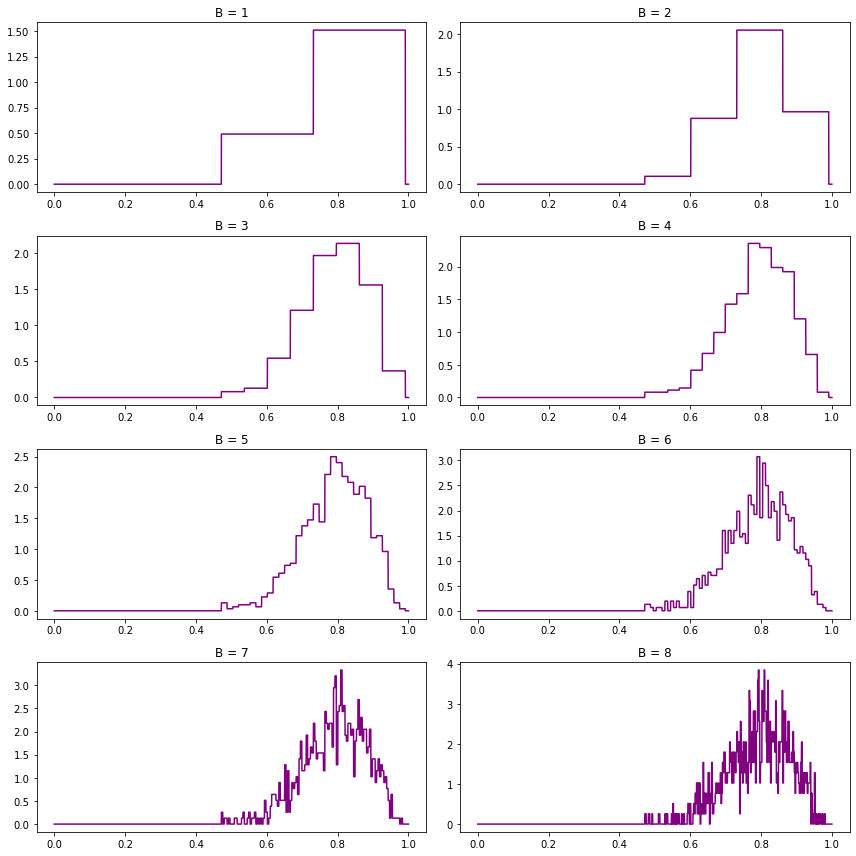
\includegraphics{Figure-22-16}
\end{figure}

Rather than using the risk expression from (c), we will use the
leave-one-out cross-validation score, as in definition 21.15:
\[
\hat{J} = \int \left( \hat{f}(x) \right)^{2} dx - \frac{2}{n} \sum_{i=1}^{n} \hat{f}_{(-i)} (X_{i})
\]
where \(\hat{f}\) is the estimator using all data, and
\(\hat{f}_{(-i)}\) is the estimator dropping the \(i\)-th observation.

\begin{python}
def leave_one_out_risk_score(X, B):
    estimator = lambda data: haar_histogram(data, B)
    
    n = len(X)
    f_hat = estimator(X)
    
    step = 1e-4
    X_min, X_max = X.min(), X.max()
    xx = np.arange(X_min, X_max + step, step)
    return (np.sum(f_hat(xx)**2) * step) \
        - (2 / n) * np.sum([estimator(X[np.arange(n) != i])(X[i]) for i in range(n)])
\end{python}

\begin{python}
# Explicitly compute risk score for multiple B values
max_B = 8
risk_B = np.empty(max_B)
for B in range(1, max_B + 1):
    risk_B[B - 1] = leave_one_out_risk_score(X, B)
selected_B = np.argmin(risk_B) + 1
selected_B_score = risk_B[selected_B - 1]
\end{python}

\begin{python}
# Plot risks and selected B value
plt.figure(figsize=(12, 8))
plt.plot(range(1, max_B + 1), risk_B)
plt.xlabel('B')
plt.ylabel(r'Risk score $\hat{J}$')
plt.show()
print('Selected B: %i' % selected_B)
print('Selected risk score: %.3f' % selected_B_score)
\end{python}

\begin{figure}[H]
\centering
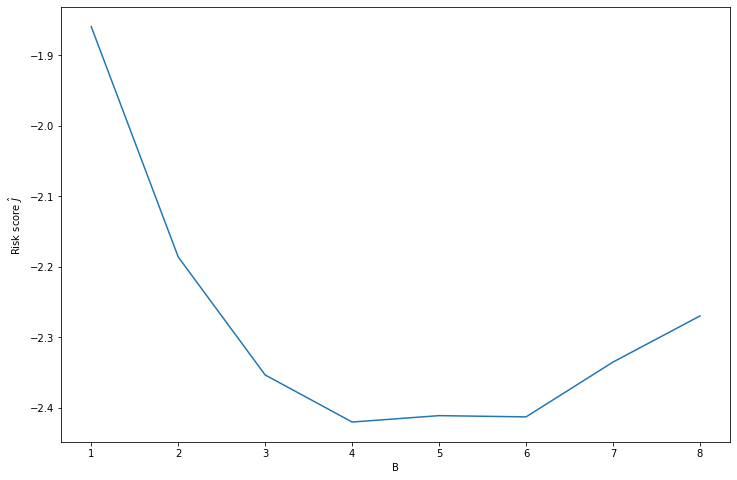
\includegraphics{Figure-22-17}
\end{figure}

\begin{console}
Selected B: 4
Selected risk score: -2.420
\end{console}

\begin{python}
f_hat = haar_histogram(X, B=selected_B)
plt.figure(figsize=(12, 8))
plt.plot(xx, f_hat(xx), color='purple')
plt.title('B = %i (min risk)' % selected_B)
plt.xlabel('X')
plt.ylabel(r'Risk score $\hat{J}$')
plt.show()
\end{python}

\begin{figure}[H]
\centering
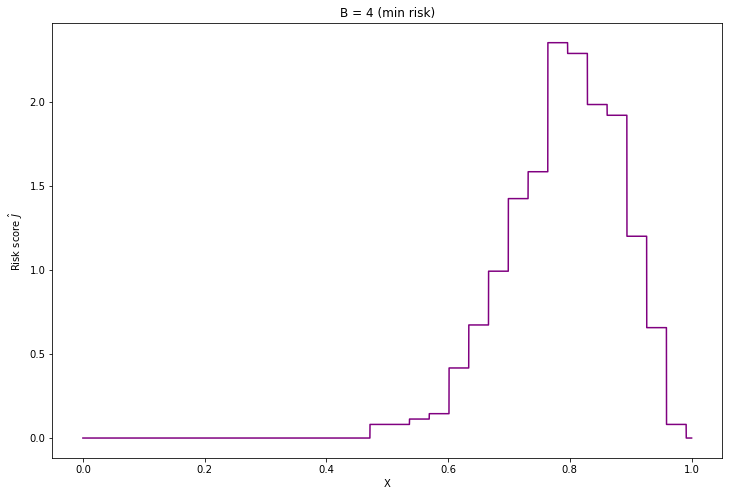
\includegraphics{Figure-22-18}
\end{figure}


\textbf{Exercise 22.6.11}. In this exercise, we will explore the
motivation for equation (22.38). Let
\(X_{1}, \dots, X_{n} \sim N(0, \sigma^{2})\). Let
\[
\hat{\sigma} = \sqrt{n} \times \frac{\text{median} (| X_{1}|, \dots, |X_{n}|)}{0.6745}
\]
\textbf{(a)} Show that \(\EXP(\hat{\sigma}) = \sigma\).
\textbf{(b)} Simulate \(n = 100\) observations from a \(N(0, 1)\)
distribution. Compute \(\hat{\sigma}\) as well as the usual estimate of
\(\sigma\). Repeat 1000 times and compare the MSE.
\textbf{(c)} Repeat (b) but add some outliers to the data. To do this,
simulate each observation from a \(N(0, 1)\) with probability .95 and
simulate each observation from a \(N(0, 10)\) with probability 0.05.

\textbf{Solution}.
\textbf{(a)} This formula seems incorrect as is -- there is no need to
rescale by \(\sqrt{n}\).
From the Median Theorem,
\(\EXP(\text{median}( \{ |X_{i}| : i = 1, \dots, n \} )) = \EXP(\text{median}(|X|))\),
where \(X \sim N(0, \sigma^{2})\). But the half normal distribution has
CDF \(F(x) = \text{erf}\left(\frac{x}{\sigma \sqrt{2}}\right)\), so the
median is
\(F^{-1}\left(\frac{1}{2}\right) = \frac{\sigma \sqrt{2}}{\sqrt{\pi}} \approx 0.6745 \sigma\).
Therefore, \(\EXP(\hat{\sigma}) = \sigma\).
\textbf{(b)}

\begin{python}
import numpy as np
from scipy.stats import norm
def run_experiment(n=100, B=1000):
    median_sigma_hat = np.empty(B)
    sd_sigma_hat = np.empty(B)
    
    for i in range(B):
        X = norm.rvs(size=n)
        median_sigma_hat[i] = np.median(np.abs(X)) / 0.6745
        sd_sigma_hat[i] = X.std()
    
    return median_sigma_hat, sd_sigma_hat
\end{python}

\begin{python}
median_sigma_hat, sd_sigma_hat = run_experiment(n=100, B=1000)
\end{python}

\begin{python}
print('E[Median sigma hat]:\t %.3f' % median_sigma_hat.mean())
print('E[SD sigma hat]:   \t %.3f'  % sd_sigma_hat.mean())
print('SE[Median sigma hat]:\t %.3f' % median_sigma_hat.std())
print('SE[SD sigma hat]:\t %.3f'     % sd_sigma_hat.std())
\end{python}
\begin{console}
E[Median sigma hat]:     1.004
E[SD sigma hat]:         0.994
SE[Median sigma hat]:    0.117
SE[SD sigma hat]:        0.072
\end{console}
As expected, both methodologies produce similar estimates for
\(\sigma\), but the median estimate has a wider variance.
\textbf{(d)}

\begin{python}
import numpy as np
from scipy.stats import norm
def run_experiment(n=100, B=1000):
    median_sigma_hat = np.empty(B)
    sd_sigma_hat = np.empty(B)
    
    for i in range(B):
        X1 = norm.rvs(size=n, scale=1)
        X2 = norm.rvs(size=n, scale=10)
        X = np.where(np.random.uniform(size=n) < 0.95, X1, X2)
        median_sigma_hat[i] = np.median(np.abs(X)) / 0.6745
        sd_sigma_hat[i] = X.std()
    
    return median_sigma_hat, sd_sigma_hat
\end{python}

\begin{python}
median_sigma_hat, sd_sigma_hat = run_experiment(n=100, B=1000)
\end{python}

\begin{python}
print('E[Median sigma hat]:\t %.3f' % median_sigma_hat.mean())
print('E[SD sigma hat]:   \t %.3f'  % sd_sigma_hat.mean())
print('SE[Median sigma hat]:\t %.3f' % median_sigma_hat.std())
print('SE[SD sigma hat]:\t %.3f'     % sd_sigma_hat.std())
\end{python}
\begin{console}
E[Median sigma hat]:     1.059
E[SD sigma hat]:         2.294
SE[Median sigma hat]:    0.122
SE[SD sigma hat]:        0.738
\end{console}
The presence of 5\% of outliers has significantly thrown off the usual
estimate for \(\sigma\), while having a smaller effect on the median
methodology.

\textbf{Exercise 22.6.12}. Repeat question 6 using the Haar basis.

\textbf{Solution}.
As in question 6, (a) and (b) are to be solved analytically, while (c)
and (d) numerically. Plots are to be provided for all scenarios.
\textbf{(a)} \(f(x) = \sqrt{2} \cos (3 \pi x)\)
We have:
\begin{align*}
\alpha &= \int_{0}^{1} f(x) \phi(x) dx = \int_{0}^{1} \sqrt{2} \cos (3 \pi x) dx = 0 \\
\beta_{j, k} &= \int_{0}^{1} f(x) \psi_{j, k}(x) dx \\
&= 2^{(j + 1)/2} \left( \int_{\frac{k + 1/2}{2^{j}}}^{\frac{k + 1}{2^{j}}} \cos(3 \pi x) dx - \int_{\frac{k}{2^{j}}}^{\frac{k + 1/2}{2^{j}}} \cos(3 \pi x) dx \right) \\
&= \frac{2^{(j + 1)/2}}{3 \pi} \left(
 \sin\left( \frac{3\pi k}{2^{j}} \right)
 + \sin\left( \frac{3\pi (k + 1)}{2^{j}} \right)
 -  2 \sin\left( \frac{3\pi \left(k + \frac{1}{2}\right)}{2^{j}} \right) 
\right)
\end{align*}

\begin{python}
# Wavelet base functions
import numpy as np
def haar_father_wavelet(x):
    return np.where((x >= 0) & (x < 1), 1, 0)
def haar_mother_wavelet(x):
    return np.where((x >= 0) & (x < 1), np.where(x <= 1/2, -1, 1), 0)
def psi_wavelet(j, k):
    def f(x):
        return 2**(j / 2) * haar_mother_wavelet((2**j)*x - k)
    return f
\end{python}

\begin{python}
alpha = 0
def beta(j, k):
    return (2**((j + 1)/2) / (3 * np.pi)) *  \
            (np.sin(3 * np.pi * k / 2**(j)) + np.sin(3 * np.pi * (k + 1) / 2**(j)) \
             - (2 * np.sin(3 * np.pi * (k + 1/2) / 2**(j)) ))
def partial_sum(B, xx):
    result = alpha * np.ones_like(xx)
    for j in range(B+1):
        for k in range(2**j):
            result += beta(j, k) * psi_wavelet(j, k)(xx)
    return result
\end{python}

\begin{python}
# Plot in separate boxes for ease of visualization
import matplotlib.pyplot as plt
%matplotlib inline
step = 1e-4
epsilon = 1e-12  # small shift to avoid spikes
xx = np.arange(0, 1, step) + epsilon
plt.figure(figsize=(12, 12))
def do_subplot(index, xx, yy, label, color):
    ax = plt.subplot(4, 1, index)
    ax.plot(xx, yy, label=label, color=color)
    ax.legend()    
do_subplot(1, xx, partial_sum(2, xx), label=r'$B = %i$' % 2, color='C0')
do_subplot(2, xx, partial_sum(4, xx), label=r'$B = %i$' % 4, color='C1')
do_subplot(3, xx, partial_sum(6, xx), label=r'$B = %i$' % 6, color='C2')
do_subplot(4, xx, np.sqrt(2) * np.cos(3 * np.pi * xx), 
           label=r'$f(x) = \sqrt{2} \cos(3 \pi x)$', color='C3')
    
plt.tight_layout()
plt.legend()
plt.show()
\end{python}

\begin{figure}[H]
\centering
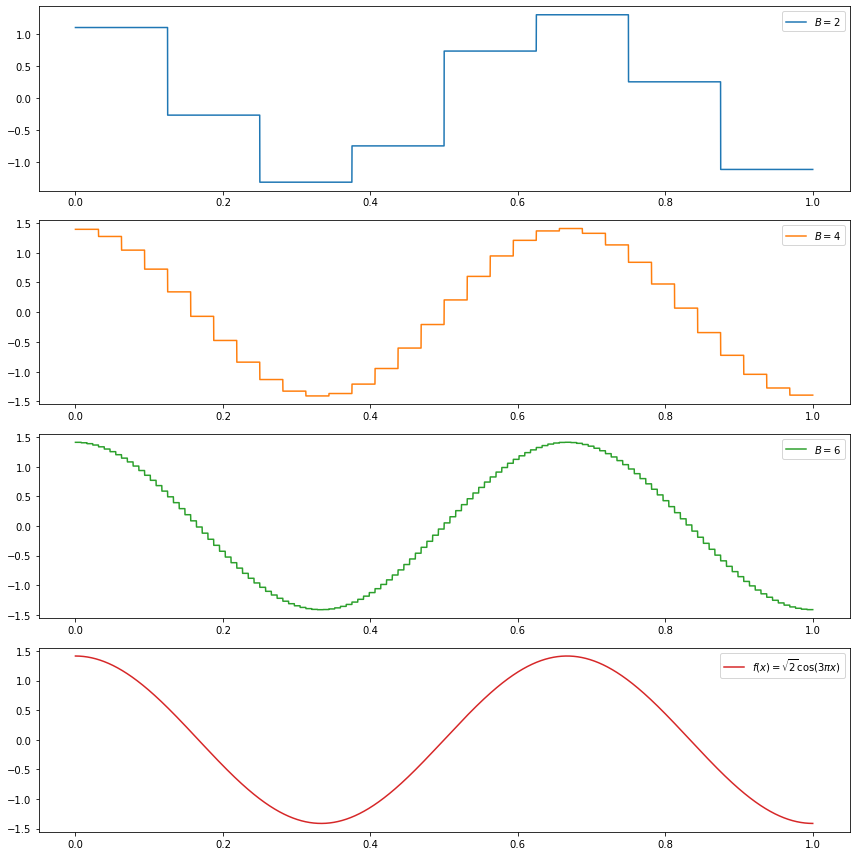
\includegraphics{Figure-22-19}
\end{figure}

\textbf{(b)} \(f(x) = \sin(\pi x)\)
We have:
\begin{align*}
\alpha &= \int_{0}^{1} f(x) \phi(x) dx = \int_{0}^{1} \sin (\pi x) dx = \frac{2}{\pi} \\
\beta_{j, k} &= \int_{0}^{1} f(x) \psi_{j, k}(x) dx \\
&= 2^{j/2} \left( \int_{\frac{k + 1/2}{2^{j}}}^{\frac{k + 1}{2^{j}}} \sin(\pi x) dx - \int_{\frac{k}{2^{j}}}^{\frac{k + 1/2}{2^{j}}} \sin(\pi x) dx \right) \\
&= \frac{2^{j/2}}{\pi} \left(
 2 \cos\left( \frac{\pi \left(k + \frac{1}{2}\right)}{2^{j}} \right) 
 - \cos\left( \frac{\pi k}{2^{j}} \right)
 - \cos\left( \frac{\pi (k + 1)}{2^{j}} \right) 
\right)
\end{align*}

\begin{python}
# Wavelet base functions
import numpy as np
def haar_father_wavelet(x):
    return np.where((x >= 0) & (x < 1), 1, 0)
def haar_mother_wavelet(x):
    return np.where((x >= 0) & (x < 1), np.where(x <= 1/2, -1, 1), 0)
def psi_wavelet(j, k):
    def f(x):
        return 2**(j / 2) * haar_mother_wavelet((2**j)*x - k)
    return f
\end{python}

\begin{python}
alpha = 2 / np.pi
def beta(j, k):
    return (2**(j/2) / np.pi) *  \
            (2 * np.cos(np.pi * (k + 1/2) / 2**(j)) \
            - np.cos(np.pi * k / 2**(j)) - np.cos(np.pi * (k + 1) / 2**(j)))
def partial_sum(B, xx):
    result = alpha * np.ones_like(xx)
    for j in range(B+1):
        for k in range(2**j):
            result += beta(j, k) * psi_wavelet(j, k)(xx)
    return result
\end{python}

\begin{python}
# Plot in separate boxes for ease of visualization
import matplotlib.pyplot as plt
step = 1e-4
epsilon = 1e-12  # small shift to avoid spikes
xx = np.arange(0, 1, step) + epsilon
plt.figure(figsize=(12, 12))
def do_subplot(index, xx, yy, label, color):
    ax = plt.subplot(4, 1, index)
    ax.plot(xx, yy, label=label, color=color)
    ax.legend()    
do_subplot(1, xx, partial_sum(2, xx), label=r'$B = %i$' % 2, color='C0')
do_subplot(2, xx, partial_sum(4, xx), label=r'$B = %i$' % 4, color='C1')
do_subplot(3, xx, partial_sum(6, xx), label=r'$B = %i$' % 6, color='C2')
do_subplot(4, xx, np.sin(np.pi * xx), label=r'$f(x) = \sin(\pi x)$', color='C3')
plt.tight_layout()
plt.legend()
plt.show()
\end{python}

\begin{figure}[H]
\centering
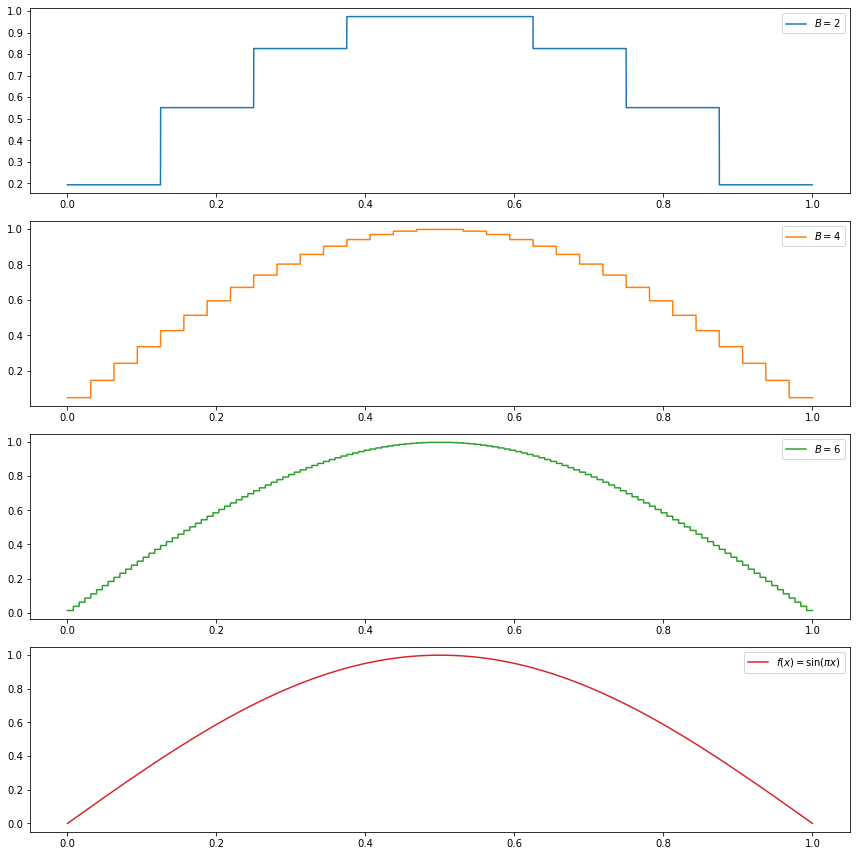
\includegraphics{Figure-22-20}
\end{figure}

\textbf{(c)} \(f(x) = \sum_{j=1}^{11} h_{j} K(x - t_{j})\), where
\(K(t) = (1 + \text{sign}(t)) / 2\),
\[
(t_{j}) = (.1, .13, .15, .23, .25, .40, .44, .65, .76, .78, .81), \\
(h_{j}) = (4, -5, 3, -4, 5, -4.2, 2.1, 4.3, -3.1, 2.1, -4.2)
\]

\begin{python}
# Wavelet base functions
import numpy as np
def haar_father_wavelet(x):
    return np.where((x >= 0) & (x < 1), 1, 0)
def haar_mother_wavelet(x):
    return np.where((x >= 0) & (x < 1), np.where(x <= 1/2, -1, 1), 0)
def psi_wavelet(j, k):
    def f(x):
        return 2**(j / 2) * haar_mother_wavelet((2**j)*x - k)
    return f
\end{python}

\begin{python}
import numpy as np
T = np.array([.1, .13, .15, .23, .25, .40, .44, .65, .76, .78, .81])
H = np.array([4, -5, 3, -4, 5, -4.2, 2.1, 4.3, -3.1, 2.1, -4.2])
def f(x):
    def K(t):
        return (1 + np.sign(t))/2
    return (H.reshape(1, -1) * K(
        x.reshape(-1, 1).repeat(len(T), axis=1) - T.reshape(-1, 1).repeat(len(x), axis=1).T)
    ).sum(axis = 1)
\end{python}

\begin{python}
N = 10000
step = 1 / N
xx = np.arange(0, 1 + step, step=step)
alpha = f(xx) @ haar_father_wavelet(xx) / N
J = 256
estimated_beta = {}
for j in range(0, 7):
    estimated_beta[j] = np.empty(2**j)
    for k in range(2**j):
        estimated_beta[j][k] = f(xx) @ psi_wavelet(j, k)(xx) / N
def beta(j, k):
    return estimated_beta[j][k]
\end{python}

\begin{python}
def partial_sum(B, xx):
    result = alpha * np.ones_like(xx)
    for j in range(B+1):
        for k in range(2**j):
            result += beta(j, k) * psi_wavelet(j, k)(xx)
    return result
\end{python}

\begin{python}
# Plot in separate boxes for ease of visualization
import matplotlib.pyplot as plt
%matplotlib inline
step = 1e-4
epsilon = 1e-12  # small shift to avoid spikes
xx = np.arange(0, 1, step) + epsilon
plt.figure(figsize=(12, 12))
def do_subplot(index, xx, yy, label, color):
    ax = plt.subplot(4, 1, index)
    ax.plot(xx, yy, label=label, color=color)
    ax.legend()    
do_subplot(1, xx, partial_sum(2, xx), label=r'$B = %i$' % 2, color='C0')
do_subplot(2, xx, partial_sum(4, xx), label=r'$B = %i$' % 4, color='C1')
do_subplot(3, xx, partial_sum(6, xx), label=r'$B = %i$' % 6, color='C2')
do_subplot(4, xx, f(xx), label=r'$f(x) = \sum_{j} h_{j} K(x - t_{j}) $', color='C3')
plt.tight_layout()
plt.legend()
plt.show()
\end{python}

\begin{figure}[H]
\centering
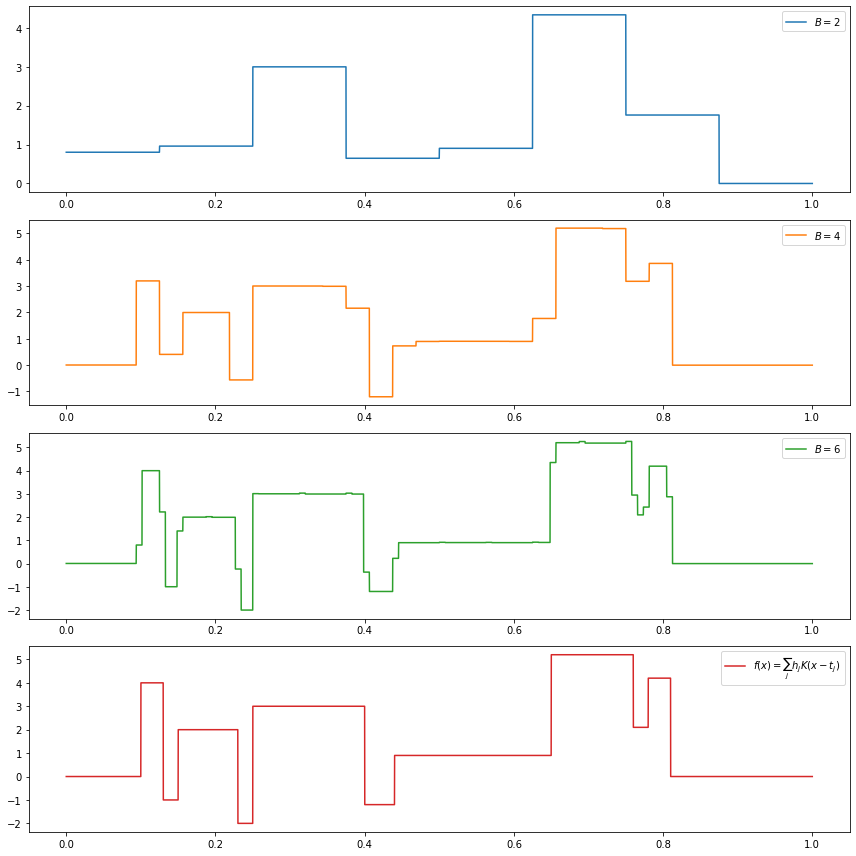
\includegraphics{Figure-22-21}
\end{figure}

\textbf{(d)} $f(x) = \sqrt{x(1-x)} \sin \left(
\frac{2.1 \pi}{(x + .05)} \right) $

\begin{python}
# Wavelet base functions
import numpy as np
def haar_father_wavelet(x):
    return np.where((x >= 0) & (x < 1), 1, 0)
def haar_mother_wavelet(x):
    return np.where((x >= 0) & (x < 1), np.where(x <= 1/2, -1, 1), 0)
def psi_wavelet(j, k):
    def f(x):
        return 2**(j / 2) * haar_mother_wavelet((2**j)*x - k)
    return f
\end{python}

\begin{python}
def f(x):
    return np.sqrt(x * (1 - x)) * np.sin(2.1 * np.pi / (x + 0.05))
\end{python}

\begin{python}
N = 10000
step = 1 / N
xx = np.arange(0, 1 + step, step=step)
alpha = f(xx) @ haar_father_wavelet(xx) / N
J = 256
estimated_beta = {}
for j in range(0, 7):
    estimated_beta[j] = np.empty(2**j)
    for k in range(2**j):
        estimated_beta[j][k] = f(xx) @ psi_wavelet(j, k)(xx) / N
def beta(j, k):
    return estimated_beta[j][k]
\end{python}

\begin{python}
def partial_sum(B, xx):
    result = alpha * np.ones_like(xx)
    for j in range(B+1):
        for k in range(2**j):
            result += beta(j, k) * psi_wavelet(j, k)(xx)
    return result
\end{python}

\begin{python}
# Plot in separate boxes for ease of visualization
import matplotlib.pyplot as plt
%matplotlib inline
step = 1e-4
epsilon = 1e-12  # small shift to avoid spikes
xx = np.arange(0, 1, step) + epsilon
plt.figure(figsize=(12, 12))
def do_subplot(index, xx, yy, label, color):
    ax = plt.subplot(4, 1, index)
    ax.plot(xx, yy, label=label, color=color)
    ax.legend()    
do_subplot(1, xx, partial_sum(2, xx), label=r'$B = %i$' % 2, color='C0')
do_subplot(2, xx, partial_sum(4, xx), label=r'$B = %i$' % 4, color='C1')
do_subplot(3, xx, partial_sum(6, xx), label=r'$B = %i$' % 6, color='C2')
do_subplot(4, xx, f(xx), 
    label=r'$f(x) = \sqrt{x (1 - x)} \sin \left( \frac{2.1 \pi}{(x + .05)} \right)$', color='C3')
    
plt.tight_layout()
plt.legend()
plt.show()
\end{python}

\begin{figure}[H]
\centering
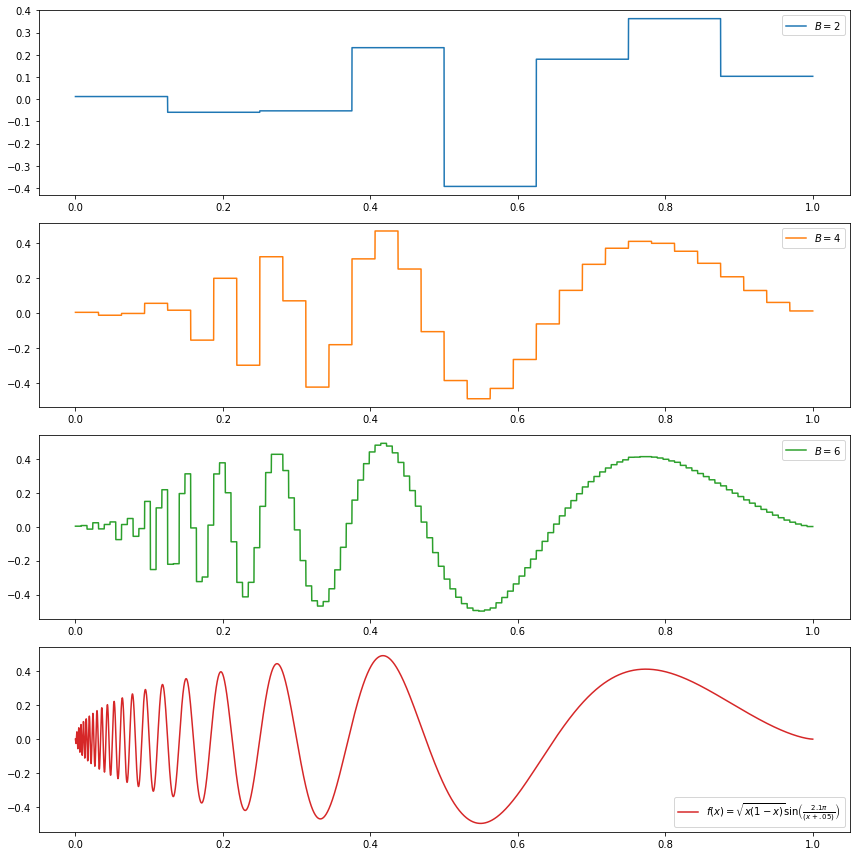
\includegraphics{Figure-22-22}
\end{figure}

